\documentclass[14pt]{extarticle}

\usepackage[utf8]{inputenc}
\usepackage[russian]{babel}
\usepackage[left=3cm, right=2.5cm, top=2cm, bottom=2cm]{geometry}
\usepackage{graphicx}
\usepackage{indentfirst} %indent first par
\usepackage{hyperref}
\usepackage[font=normalsize,labelfont=it,justification=centering]{caption} %for customize caption
\usepackage{float} %for figure position
\usepackage{amsmath} %for math equations

\def\UrlBreaks{\do\/\do\-\do\_\do\%\do\.} %for cutting urls

\usepackage{xr}		% for cross-file references
\externaldocument{main} %

\usepackage{enumitem} %for list customization
\setlist[itemize]{leftmargin=2cm,labelsep=0.5cm}
\setlist[enumerate]{leftmargin=1.5cm}

\usepackage{pscyr} %russian fonts
\renewcommand{\rmdefault}{ftm}

\tolerance=1200

\graphicspath{ {./images/} }

\pagestyle{plain} %for counting pages
\setcounter{page}{2}

\parindent=1.5cm %paragraph style
%\linespread{1.3}

\newcommand{\specialcell}[2][c]{%command \specialcell for auto-carry in cells of table
\begin{tabular}[#1]{@{}c@{}}#2\end{tabular}}
\usepackage{caption}
\captionsetup[table]{justification=raggedright, singlelinecheck=false} %table caption left align

\usepackage{titlesec}
\titleformat*{\section}{\large\bfseries}
\titleformat*{\subsection}{\normalsize\bfseries}
\titleformat*{\subsubsection}{\normalsize\bfseries}
\titleformat*{\paragraph}{\normalsize\bfseries}
\titleformat*{\subparagraph}{\normalsize\bfseries}

\usepackage{listings} %listings
\usepackage{color} %colors for listings
\definecolor{dkgreen}{rgb}{0,0.6,0}
\definecolor{gray}{rgb}{0.5,0.5,0.5}
\definecolor{mauve}{rgb}{0.58,0,0.82}	
\lstset{ 
  backgroundcolor=\color{white},   % choose the background color; you must add \usepackage{color} or \usepackage{xcolor}; should come as last argument
  basicstyle=\footnotesize\ttfamily,        % the size of the fonts that are used for the code
  breakatwhitespace=false,         % sets if automatic breaks should only happen at whitespace
  breaklines=true,                 % sets automatic line breaking
  captionpos=b,                    % sets the caption-position to bottom
  commentstyle=\color{dkgreen},    % comment style
  deletekeywords={...},            % if you want to delete keywords from the given language
  escapeinside={\%*}{*)},          % if you want to add LaTeX within your code
  extendedchars=\true,              % lets you use non-ASCII characters; for 8-bits encodings only, does not work with UTF-8
  firstnumber=1,                % start line enumeration with line 1000
  frame=single,	                   % adds a frame around the code
  keepspaces=true,                 % keeps spaces in text, useful for keeping indentation of code (possibly needs columns=flexible)
  keywordstyle=\color{blue},       % keyword style
  language=C++,                 % the language of the code
  morekeywords={*,...},            % if you want to add more keywords to the set
  numbers=left,                    % where to put the line-numbers; possible values are (none, left, right)
  numbersep=14pt,                   % how far the line-numbers are from the code
  numberstyle=\footnotesize\color{black}, % the style that is used for the line-numbers
  rulecolor=\color{black},         % if not set, the frame-color may be changed on line-breaks within not-black text (e.g. comments (green here))
  showspaces=false,                % show spaces everywhere adding particular underscores; it overrides 'showstringspaces'
  showstringspaces=false,          % underline spaces within strings only
  showtabs=false,                  % show tabs within strings adding particular underscores
  stepnumber=1,                    % the step between two line-numbers. If it's 1, each line will be numbered
  stringstyle=\color{mauve},     % string literal style
  tabsize=2,	                   % sets default tabsize to 2 spaces
  title=\relax,                   % \lstname show the filename of files included with \lstinputlisting; also try caption instead of title
  inputpath=listings, %relative path to the listings,
  xleftmargin=5.0ex, % left indent
  belowskip=-2.5em,
  aboveskip=0.5em,
  inputencoding=utf8
}

%\sloppy sparse auto-carry strings

\begin{document}
	\include{description} %incorrect year!!!
	{ %tableOfContents
	\addtocontents{toc}{\protect\sloppy}

}	
\renewcommand{\contentsname}{Table of contents}
\tableofcontents{}
	{ %introduction
	\phantomsection
	\section*{Introduction}
	\addcontentsline{toc}{section}{Introduction}
	\par Currently, most microprocessors are multi-core. This applies not only to desktop computers, but also to mobile phones and tablets (so far, only embedded computing systems are an exception). To fully realize the potential of a multi-core system, a programmer needs to use special methods of parallel programming, which are becoming increasingly popular in industrial programming. However, parallel programming methods are significantly more difficult to master than traditional sequential program writing methods.
	\par The purpose of this study book is to describe practical tasks (laboratory work) that can be used to consolidate the theoretical knowledge gained as part of a lecture course on parallel programming technologies. In addition, the book summarizes the basic principles of parallel programming.%, при этом теоретический материал даётся тезисно и поэтому для полноценного освоения требуется использовать конспекты лекций по соответствующей дисциплине.
	\par While programming multi-threaded applications, you have to resolve conflicts that arise when simultaneously accessing the shared memory of several threads. The following three conceptually different approaches are currently used to synchronize simultaneous access to shared memory:
	\begin{enumerate}
		\item\textbf{Explicit use of blocking primitives}\quad(mutexes, semaphores, condition variables). This approach historically appeared first and is now the most common and supported in most programming languages. The disadvantage of this method is a rather high entry threshold, since the programmer is required to manage blocking primitives in the  "manual mode"', tracking conflict situations when accessing shared memory.
		\item\textbf{Software Transactional Memory(STM)}. This method is easier to learn and use than the previous one, however it still has limited support in compilers, and it will also be able to fully manifest itself with the wider distribution of processors with hardware support for STM.
		\item\textbf{Non-blocking algorithms}\quad(lockless, lock-free, wait-free algorithms). This method implies a complete rejection of the use of blocking primitives with the help of complex algorithmic tricks. Moreover, for the correct functioning of the non-blocking algorithm, it is required that the processor supports special atomic (conflict-free) operations of the form "compare and exchange'' (cmpxchg, "compare and swap''). Currently, most processors have this type of operation as part of the instruction system (with rare exceptions, for example: ''SPARC 32'').
	\end{enumerate}
	\par The methodological manual proposed is devoted to the first of the listed methods, since he received the greatest coverage in literature and the greatest application in industrial programming. Two other methods may be the subject of in-depth training courses on parallel computing.
%%	\parАвторы ставили целью предложить читателям изложение основных концепций параллельного программирования в сжатой форме в расчёте на самостоятельное изучение пособия в течение двух-трёх месяцев. При использовании пособия в технических вузах рекомендуется приведённый материал использовать в качестве односеместрового учебного курса в рамках %бакалаврской
 %%подготовки студентов по направлению подготовки ''Программная инженерия'' или смежных с ней.% Однако приводимые примеры практических заданий могут быть при желании адаптированы для использования в магистерских курсах.

}
	{ %section1
	\section{Theoretical Foundations of Parallel Computing}
	{ %section1_1
	\subsection{History of parallel computing}
	\par Conversation about the development of parallel computing is usually begun with the history of the development of supercomputers. However, the world's first supercomputer CDC6600, created in 1963, had only one central processor, so it can hardly be considered a full-fledged SMP system.
	\par The third-ever CDC8600 supercomputer was designed to use four processors with shared memory, which suggests the first use of SMP, but the CDC8600 was never released since its development was discontinued in 1972.
	\par Only in 1983 was it possible to create a working supercomputer (Cray X-MP), which used two central processors that used shared memory. It is worth noting that a little earlier (in 1980) the first Russian multiprocessor computer Elbrus-1 appeared, however, it was significantly inferior in performance to supercomputers of that time.
	\par Already in 1994 it was possible to freely buy a desktop computer with two processors, when ASUS released its first motherboard with two sockets - connectors for installing processors.
	\par The next step in the development of SMP-systems was the emergence of multi-core processors. The first multi-core processor for mass use was POWER4, released by IBM in 2001. But the truly widespread multi-core architecture received only in 2005, when AMD and Intel released their first dual-core processors.
	\par The Figure~\ref{GraphPartOfMultiCoreProcessorFromYear:image} shows how much CPU with a different number of cores occupied when creating supercomputers at different times (according to the materials of the site (\url{http://top500.org}). Закрашенные области помечены цифрами 1, 2, 4, 6, 8, 10, 12, 16 для обозначения количества ядер. Ширина области по вертикали равна относительной частоте использования процессоров соответствующего типа в рассматриваемом году.
	\begin{figure}[H]
		\includegraphics[width=1\linewidth]{GraphPartOfMultiCoreProcessorFromYear}
		\caption{\textit{Frequency of using processors with different number of cores when creating supercomputers}}
		\label{GraphPartOfMultiCoreProcessorFromYear:image}
	\end{figure}
	\par As you can see, the active use of dual-core processors in supercomputers began already in 2002, and by about 2005 completely disappeared, whereas in desktop computers their use was only just beginning in 2005. Based on this, you can make a simple forecast of the prevalence of multi-core "desktop" processors by the desired year, if we assume that they in general outline repeat the development of multi-core architectures of supercomputers.
	\par
}
	{ %section1_2
	\subsection{Terms and Definitions}
	\par\textbf{Parallel computing} – 
A method of organizing calculations in which the program is a set of interacting modules that work simultaneously. Typically, the concept of concurrency may include:
		\begin{enumerate}
			\item\textbf{Instruction level parallelism} - one processor core can execute several instructions simultaneously. For example, this technology is implemented in Intel Pentium 4 processors.
			\item\textbf{Hypertreading} - one processor core is designed so that it can do the work of two threads at once. Implemented in the Intel Core i7 series processors. When performing laboratory work, it is important to disable this in the BIOS (if the processor is compatible with this technology), since it significantly affects the performance of parallel acceleration and efficiency.
			\item\textbf{Multi core programming} -  a method for solving computational problems with simultaneous execution of program parts on different physical computing cores. All cores have shared memory banks, as they are located on the same computer. It includes the case of a multi-core processor architecture and a multi-processor architecture of a system in which there are several processors, since in both cases the program runs on several cores of one or many processors, but on one physical computer.
			\item\textbf{Distributed computing} -a way to solve time-consuming computing problems using several computers, most often combined into a parallel computing system. Different parts of the program can run on different computers.
		\end{enumerate}
Usually the last two concepts are physically implemented using architectures. \textit{SMP} и \textit{MMP}. More details about these architectures can be found in the next section.
	\par It is important to see difference between the concepts of parallel compu-ting and parallel technologies. Let  analyze the following concepts, which, although they are parallel technologies (at the core or internuclear interaction level), however, are not parallel calculations, but often \ textbf {by mistake} are assigned to them:
		\begin{itemize}
			\item\textit{Pipeline data processing (superscalarity)} represents the simultaneous processing by the processor of several instructions, in which at one time for each of the instructions a different execution step is performed. For example, if any processor can simultaneously receive, decode, and execute an instruction, then when it receives the first instruction, it can decode the second and execute the third (Figure~\ref {pipelineExample:image}). This way of organizing calculations is not parallel computing, because the instructions are still executed sequentially, and only one core is involved.
				\begin{figure}[H]
					\includegraphics[width=1\linewidth]{pipelineExample}
					\caption{\textit{Instruction pipelining}}
					\label{pipelineExample:image}
				\end{figure}
			\item\textit{SIMD-etensions (MMX, SSE)} provide concurrency at the data level. For example, a processor can simultaneously multiply 4 numbers instead of one using the SSE instruction. However, the command flow still remains single, i.e. one program instruction is executed in a period of time, which is not the case of parallel computing.
			\item\textit{Preemptive Multitasking} organized by the operating system. Several processes are in the execution queue and the OS decides how to manage the processor time between them. If the first thread is given a higher priority than the second, then the OS will allocate more time to execute the first thread, only one thread will be executed at a time, therefore, preemptive multitasking is also not included in the concept of parallel computing.
		\end{itemize}
	\par Various parallelization technologies are used to organize parallel computing:
		\begin{itemize}
			\item\textbf{Process} - the most heavyweight mechanism used for parallelization. Each process has its own independent address space, so data synchro-nization between processes is long and complicated. May include several threads of execution.
			\item\textbf{Thread} It runs independently of other threads, but has a common address space with other threads in the same process. At this level, data synchronization mechanisms are used (will be discussed later).
			\item\textbf{Fiber} - lightweight thread of execution. Like threads, fiber has a common address space, however, it uses joint multitasking instead of preemptive one. The OS does not switch the context from one thread to another, instead, the main thread itself allocates time for the child fiber to work, or is blocked logically (that is, the programmer controls the fiber life cycle). Also, all fibers work on one core, unlike threads, which can work on different kernels.
		\end{itemize}
	\par For a better understanding of threads, we will schematically consider its life cycle. Figure ~\ref{threadLifecycle:image} shows that the flow can be in three states - readiness, expectation and fulfillment. After creating the thread, it is in a ready state. Then, the OS decides to change its state (clarifying multitasking). For fiber, the life cycle is the same, but the programmer or synchronization mechanisms control the transitions between them.
	\par Different standards of programming languages can add new states to the life cycle of threads, for example, blocking a thread, interrupting a thread, and others, but the general scheme of work remains the same.
		\begin{figure}[H]
			\includegraphics[width=0.9\linewidth]{threadLifecycle}
			\caption{\textit{Thread lifecycle}}
			\label{threadLifecycle:image}
		\end{figure}
	\par Among programmers there are concepts of \textbf{thread-safe} и \textbf{reentrant} functions, however, they may have different meanings in different communities. Definitions are written from various sources in Table~\ref{threadSafeReentrant:table}.
	\begin{table}[H]
		\caption{Definitions of thread-safe and reentrant functions}
		\label{threadSafeReentrant:table}
		\begin{center}
			%\begin{tabular}{c}
				%\begin{figure}[H]
					\includegraphics[width=1\linewidth]{parallelFunctionTypes}
				%\end{figure}
			%\end{tabular}
		\end{center}
	\end{table}
	\par Consider examples of functions that fit the definition of the Linux community.
	\begin{figure}[H]
		\lstinputlisting{swapExample1.cpp}
	\end{figure}
	\par This function is not thread safe, not reentrant, because all threads calling it will use the common variable t. If you call the function inside itself, then the value of t is overwritten and the parent function will not work correctly. Let's try to fix these errors by declaring a variable of type t \textunderscore \textunderscore threadint.
	\begin{figure}[H]
		\lstinputlisting{swapExample2.cpp}
	\end{figure}
	\par Now the compiler will create a copy of the variable for each thread t and the function will become thread safe, however, it is still not reentrant for the same reason. We will save the value of the global variable t at the beginning of the function and restore it at the end.
	\begin{figure}[H]
		\lstinputlisting{swapExample3.cpp}
	\end{figure}
	\par The new function is reentrant, but again non thread-safe. Finally, we give an example of a standard and proper implementation of \texttt{swap()}, which is thread safe and reentrant:
	\begin{figure}[H]
		\lstinputlisting{swapExample4.cpp}
	\end{figure}
}
	{ %section1_3
	\subsection{Classification of parallel systems (architectures)}
	\par By physical architecture, parallel systems can be divided into 2 types:
		\begin{enumerate}
			\item\textbf{SMP} (Shared Memory Parallelism, Symmetric MultiProcessor system)~– multiprocessing, multicore, GPGPU. 
			\item\textbf{MPP} (Massively Parallel Processing) – cluster systems, GRID (distributed computing).
		\end{enumerate}
	\par We consider these two architectures in more detail.
	\par\textbf{\textit{SMP}} – architecture of multiprocessor systems in which two or more identical processors of comparable performance are connected in the same way to the shared memory (and peripheral devices) and perform the same functions (why, in fact, the system is called symmetrical). SMP systems are also called tightly coupled multiprocessors, since in this class of systems processors are closely connected to each other via a common bus and have equal access to all resources of the computing system (memory and input-output devices) and are controlled by all one copy of the operating system. In this architecture, all processors are located on the same physical machine, so they have common memory banks. There are two types of connecting processors to shared memory:
		\begin{itemize}
			\item The connection on the system bus is shown in the Figure~\ref{SMPSystemBus:image}. In this case, only one processor can access memory at any given moment, which imposes a significant limitation on the number of processors supported in such systems. The more processors, the greater the load on the shared bus, the longer each processor must wait until the bus is free to access the memory. A decrease in the overall performance of such a system with an increase in the number of processors occurs very quickly, therefore, usually in such systems the number of processors does not exceed 2-4. An example of SMP machines with this method of connecting processors is any entry-level multiprocessor server.
				\begin{figure}[H]
					\includegraphics[width=1\linewidth]{SMPSystemBus}
					\caption{\textit{SMP architecture. Processor connection via system bus}}
					\label{SMPSystemBus:image}
				\end{figure}
			\item The crossbar switch is shown in the Figure~\ref{SMPCrossbarSwitch:image}. With this connection, the entire shared memory is divided into memory banks, each memory bank has its own bus, and the processors are connected to all buses, having access to any of the memory banks through them. Such a connection is technologically more complex, but it allows processors to access shared memory at the same time. This allows you to increase the number of processors in the system to 8-16 without a noticeable decrease in overall performance.
				\begin{figure}[H]
					\includegraphics[width=1\linewidth]{SMPCrossbarSwitch}
					\caption{\textit{SMP architecture. Processor connection via dial-up connection}}
					\label{SMPCrossbarSwitch:image}
				\end{figure}
		\end{itemize}
	\par The advantages of this approach are the high speed of data exchange between processors and the relative simplicity of software development. However, there may be problems with the scalability of the system (if there are only 2 sockets on the motherboard, you can’t put 3 processors anymore).
	\par\textbf{\textit{MMP}} - architecture of multiprocessor systems, in which the memory between the processors is physically divided. On such systems, distributed computing is performed. The system is built from separate nodes containing a processor, a local memory bank, communication processors or network adapters, sometimes hard drives and other input-output devices. Access to the memory bank of this node is available only to processors from the same node. The nodes are connected by special communication channels (Figure~\ref{MMP:image}).
		\begin{figure}[H]
			\includegraphics[width=1\linewidth]{MMP}
			\caption{\textit{MMP Architecture}}
			\label{MMP:image}
		\end{figure}
	\par The advantages of this approach are its good scalability (if necessary, to increase system performance it is enough to simply add more nodes). However, the speed of interprocessor exchange is significantly reduced, since memory banks are now physically separated. Also, the cost of the software that distributes the calculations is very high.
	\par
}
	{ %section1_4
	\par In parallel programs, the developer often faces the problem of synchronization between threads. As a rule, problems arise when accessing memory and at the same time executing some critical sections of code - critical sections.
	\par\textbf{Critical area} is the section of the program, which must be executed with the exclusive right of access to shared data referenced in this program. A process preparing to enter a critical area may be delayed if any other process is in progress at that time in a similar critical area. 
	\par This section will discuss in detail thread synchronization mechanisms at the program level.
	\par The following methods are available for solving thread synchronization problems:
		\begin{itemize}
			\item\textbf{Atomic operations} are operations that are performed in their entirety or not at all. For example, a transaction to a database is an atomic operation. When two threads try to increment the same memory cell out of sync, the value can increase by 2, or maybe 1, depending on the behavior of the threads, since the increment operation is at least 3 assembler instructions. To avoid this, it is worth declaring the data type atomic (if there is one in this programming language / library). A special case of atomic operations is read-modify-write operations: compare-and-swap, test-and-set, fetch-and-add. The problem of the implementation of atomic operations will be raised in more detail in the section.\\~\ref{atomic:section} \textit{Atomic operations in a multithreaded program}.
			\item\textbf{Semaphore} - an object that limits the number of threads that can enter this area of code. Typically, this number is set when the semaphore is initialized. Then, when capturing a semaphore by a thread, the number of threads that captured the semaphore is checked. If the maximum number of threads is reached, then the thread will wait until some of the threads that entered the code area release it. Often the use of semaphores is unjustified, since the overhead of creating and maintaining a semaphore is large. You should also avoid the "semaphore leak" a situation in which the thread does not exit the semaphore when the code area completes execution if the programmer forgot to free the resource.
			\item\textbf{Reader/writer semaphore} пives the threads \textit{only} read or write permissions, and while writing data to one thread, the rest of the threads do not have access to the resource. However, in such semaphores there may be a problem \textit{resource starvation}, in which while streams will read data, other streams will not be able to write data for a long period of time or vice versa. A particular solution to this problem with equal priority of threads can be sequential access of threads in the queue to access and write.
			\item\sloppy{\textbf{Mutex} is a special case of a semaphore, in which only one thread can capture a given area of code. If the mutex serves several critical sections, only one thread can be in any of the critical sections. It is often used in the organization of critical section management, since it is "lighter" than the classical semaphore (it is enough to store one boolean variable instead of a counter), but unlike it, it is assumed that the same stream will capture and release the mutex. It should be noted that in the C++11, in addition to the standard mutex, there are various modifications of it: \textit{recursive\textunderscore mutex} - mutex that allow re-entry into the critical section by the same stream.  \textit{timed\textunderscore mutex} - мmutex with capture timer, and \textit{recursive\textunderscore timed\textunderscore mutex}, combining the advantages of both versions.}
			\item\textbf{Spinlock} is a  lock in which a thread in a loop waits for a resource to free. It is not always the optimal solution, since the waiting thread works while waiting. Inside the code section, thread interruptions must be avoided to avoid deadlock.
			\item\textbf{Seqlock} - synchronization mechanism designed to quickly record a variable in multiple threads. The Linux kernel works as follows: the thread waits until the critical section is released (spinlock); when entering the section, the counter increments, the stream does its work. When exiting a section, the flow checks the counter value. If the counter value has not changed, it means that no one has written data at the moment and the stream exits the critical section, otherwise it reads the value of the variable again.
			\item\textbf{Knuth–Bendix сompletion algorithm} - One of the solutions to synchronization problems is the Knuth-Bendix algorithm from the course of discrete mathematics. With it, you can go from a sequential program to a cascading one. However, this algorithm does not work for all programs; sometimes it can go into an infinite loop or fail.
			\item\textbf{Barier} - a part of code in which the state of threads is synchronized. For example, if a function in the main thread requires all child threads to finish their work, you can put a barrier in front of it. Then it will wait for the completion of the child threads, after which all threads will continue to work. An example of a barrier implementation may be a critical section, the code of which is allowed to be executed only by the last thread that requested execution. The rest of the threads should expect it. To do this, you need to know how many threads should come to the barrier.
			\item\textbf{Non-blocking algorithms.} It is often useful not to use standard locking techniques, but to make the algorithm non-blocking. In this case, the programmer must independently guarantee that critical sections of the code will not be executed simultaneously and the integrity of the shared memory. Another advantage of such algorithms is the safe handling of interrupts. Other synchronization technologies are often used to implement such algorithms: read-modify-write, CAS (see section~\ref{atomic:section}) and etc.
			\item\textbf{RCU (read-copy-update)} - is an algorithm that allows threads to efficiently read data, leaving the data updated at the end of the algorithm, while guaranteeing relevant data. Only one thread can write data, but multiple threads can read data at once. This is achieved, for example, by atomic pointer substitution (CAS). Old versions of the data are stored for past hits, as long as they have at least one pointer. There are newer tools for replacing the pointer: a separate deadlock for writers or the membarrier mechanism used in recent versions of Linux. RCU can be useful in organizing data structures without explicit locks.
			\item\textbf{Monitor} - An object encapsulating a mutex and utility variables to provide secure access to a method or variable by multiple threads. The monitor characterizes that at one moment only one thread can execute any of its methods. For example, if we have a class (in C ++ terms) Account with add methods\textunderscore money(),\\sub\textunderscore money(), it makes sense to make it a monitor so that there are no conflicts when conducting operations with the account.
		\end{itemize}
		\par However, it is not necessary to organize parallel computations using synchronization or locks. Some technologies offer an alternative approach to parallel computing:
		\begin{itemize}
			\item\textbf{Program Transactional Memory} - a memory model in which operations performed on memory cells are atomic. Advantages of use: ease of use (enclosing code blocks in a transaction block), lack of locks, however, if used incorrectly, performance may drop, as well as the inability to use operations that cannot be undone inside a transaction block. In the compiler, GCC is supported since version 4.7 as follows:
				\begin{enumerate}
					\item\textunderscore \textunderscore transaction\textunderscore atomic \{ … \} — an indication that the code block is a transaction;
					\item\textunderscore \textunderscore transaction\textunderscore relaxed \{ … \} — an indication that the unsafe code inside the block does not lead to side effects;
					\item\textunderscore \textunderscore transaction\textunderscore cancel — explicit transaction cancellation;
					\item attribute((transaction\textunderscore safe)) — indication of a transaction-safe function;
					\item attribute((transaction\textunderscore pure)) — indication of function without side effects.
				\end{enumerate}
			\item\textbf{Actor model} - a mathematical model of parallel computing, in which the program is an actor objects that interact with each other and can create new actors, send and send messages to each other. The parallelism of computations within one actor is assumed. Each actor has an address to which you can send a message. Each actor works in a separate thread. The actor model is used to organize email, some SOAP web services, and etc.
		\end{itemize}
	\par Despite the large number of synchronization methods, it is most often necessary to proceed from the problem being solved. For example, if we want to make a general incremental integer variable for several threads, it makes no sense to create a mutex or semaphore, it is more optimal to make the variable atomic. Always consider the overhead of creating locks and development time.
}
	{ %section1_5
	\subsection{Automatic parallelization of programs}
	\par Parallel computing is a rather complicated manual process, so it seems obvious that it needs to be automated using a compiler. Such attempts are made, however, the efficiency of auto-parallelization is not yet sufficient, because good indicators of parallel acceleration are achieved only for a limited set of simple for-cycles in which there are no data dependencies between iterations and the number of iterations cannot change after the start of the cycle. But even if the two indicated conditions are satisfied in a certain for-cycle, but it has a complex non-obvious structure, then its parallelization will not be performed. Types of automatic parallelization:
	\begin{itemize}
		\item\textit{Fully automatic:}\quad participation of the programmer is not required, all actions are performed by the compiler.
		\item\textit{Semi-automatic:}\quad programmer gives instructions to the compiler in the form of special keys that allow you to adjust some aspects of parallelization.
	\end{itemize}
	\par Weaknesses of automatic parallelization:
	\begin{itemize}
		\item erroneous change in program logic;
		\item speed reduction instead of increase;
		\item lack of manual parallelization flexibility;
		\item only cycles are efficiently parallelized;
		\item inability to parallelize programs with a complex algorithm of work.
	\end{itemize}
	\par Here are examples of how the c-program in the src.c file can be automatically parallelized using some popular compilers:
	\begin{itemize}
		\item Compiler GNU Compiler Collection:	 \\
\texttt{gcc -O3 -floop-parallelize-all -ftree-parallelize-loops=K -fdump-tree-parloops-details src.c}. \\ In this case, the programmer can choose the value of the parameter K, which is recommended to be set equal to the number of cores (processors). Features of the auto-parallelization implementation in gcc are dedicated to an independent project:\\ \url{https://gcc.gnu.org/wiki/AutoParInGCC}. 
		\item Intel compiler:	 
\texttt{icc -c -parallel -par-report file.cc}
		\item Oracle compiler:	 
\texttt{solarisstudio -cc -O3 -xautopar \\-xloopinfo src.c}
	\end{itemize}
}
	{ %section1_6
	\subsection{The main approaches to parallelization}
	\par In practice, there are a large number of parallel computing patterns. However, all these patterns basically use three basic approaches to parallelization:
	\begin{itemize}
		\item\textbf{Data parallelization:} The programmer finds in the program an array of data whose elements the program sequentially processes in some func function. Then the programmer tries to break this data array into blocks that can be processed in func independently of each other. Then the programmer starts several threads at once, each of which executes func, but at the same time processes data blocks different from other flows in this function.
		\item\textbf{Instruction parallelization:} The programmer finds in the program sequentially called functions, the process of which does not affect each other (such functions do not change common global variables, and the results of one are not used by the other). Then the programmer starts these functions in parallel threads.
		\item\textbf{Parallelization of information flows:} A program is a set of functions that can be performed, and several functions can expect the result of the previous ones. In this case, each core performs the function for which the data is already ready. Consider this method as an example of an abstract dual-core processor, as the most difficult to understand. The structural algorithm shown in the Figure~\ref{structAlgorithm:image} consists of 9 functions, some of which use the result of the previous function in their work. We assume that function 3 uses the result of the function 1, and function 7 uses the result of functions 4 and 6, etc., and also function 5 is executed in time approximately as much as functions 7, 8, and 9 combined. Then, on a dual-core machine, this parallelization method will be the optimal solution.
	\end{itemize}
	\begin{figure}[H]
		\includegraphics[width=1\linewidth]{structAlgorithm}
		\caption{\textit{An example of the operation of a structural algorithm on a dual-core processorе}}
		\label{structAlgorithm:image}
	\end{figure}
	\par The three methods described are easier to understand by analogy from everyday life. Let two students in the construction team be given the task of sweeping the street and painting the fence. If students decide to use data parallelization, he will first sweep the street together, and then paint the fence together. If they decide to use parallelization according to the instructions, then one student will completely sweep the street, and the other will paint the entire fence at this time. This situation cannot be parallelized over the information flows, since these two actions are in no way dependent on each other. If we assume that they both need tools for work, then one of them must first go after them, and then both of them will begin to do their work.
	\par In more cases, the decision to use the method is obvious due to the internal features of the parallelized program. The choice of method is determined by which one loads flows more evenly. Ideally, all threads should finish the work allocated to them approximately at the same time in order to optimally load the kernels (processors) and so that the threads that have finished their work do not stand idle while waiting for the completion of work by neighboring threads.
	\par
}
	{ %section1_7
	\subsection{Atomic operations in a multithreaded program}
	\label{atomic:section}
	\par The main problem with parallel computing is the need to resolve conflicts while accessing the shared memory of several threads. To solve this problem, they usually try to streamline the access of streams to shared data using special tools - synchronization primitives. However, the question arises whether there are such atomic atomic operations, the execution of which by several threads simultaneously does not require synchronization of actions, because these operations would be performed by the processor in one fell swoop, or, as they say, atomically (i.e., no other operation can push the previous atomic operation out of the processor before it is completed).
	\par Almost all assembler instructions are such operations, since at a low level they use only those operations that are present in the processor command system, which means that they can be performed atomically (uninterruptedly). However, when compiling a C program, C language commands are usually translated into several assembler instructions. In this regard, the question arises about the possible existence of C-commands that are compiled into one assembler instruction. Such commands could not be "protected"\ by synchronization primi-tives (mutexes) in parallel computing.
	\par However, there are very few such operations, and some of them can behave both atomically and non-atomically depending on the hardware platform for which the C program is compiled. Consider the simplest increment command of an integer variable (int type) in C: \texttt{"w++"}. You can easily verify (for example, using the gcc compiler's \texttt{"\--S"}\ key) that this command will be translated into three assembler instructions (take from memory, increase, put back):
	\begin{figure}[H]
		\lstinputlisting[language={[x86masm]Assembler}]{atomicOperationExample1.asm}
	\end{figure}
	\par This means that it is not safe to perform the increment operation of a variable in several threads at the same time, because when executing assembler instruction 2, the thread can be interrupted and the processor transferred to another thread, which will receive an incorrect value of the undereduced variable.
	\par It is logical to assume that assignment operations should not have the described problem. Indeed, in Assembler there is a separate instruction for writing the value of a variable to the specified address. Unfortunately, this assumption is not completely true: when assigning a variable of type char, this operation will be performed by a single assembler instruction. However, with other data types this cannot be said for sure. The general rule of thumb can be roughly stated as follows: "the atomicity of the assignment operation is guaranteed only for operations with data whose bit capacity does not exceed the processor bit capacity."
	\par For example, when assigning an int variable to a 32-bit processor, one assembler instruction will be generated. However, when compiling the same operation on a 16-bit computer, two assembler instructions will be generated to write the low and high bits independently.
	\par The formulated rule works with the assignment of variables and expressions, however, it cannot always be satisfied with the assignment of constants. Consider an example of C-code in which a 64-bit variable s (type uint64 \textunderscore t) is assigned a large number, obviously exceeding the 32-bit value:
	\begin{figure}[H]
		\lstinputlisting{atomicOperationExample2.cpp}
	\end{figure}
	\par This code will be translated into the following assembler code on a 64-bit processor:
	\begin{figure}[H]
		\lstinputlisting[language={[x86masm]Assembler}]{atomicOperationExample3.asm}
	\end{figure}
	\par As you can see, the assignment operation was translated into two assemb-ler instructions, which makes it impossible to safely parallelize such an operation.
	\par This rule applies not only to the assignment operation, but also to the operation of reading a variable from memory, so any of these operations in a thread-safe environment will have to be protected by mutexes or critical sections.
	\par A special case of atomic data changes is structure changes. To do this, we need to use a CAS operation with a pointer to this structure. Performing such an operation, the processor will create a second data structure with the specified fields and compare it with the old version of the structure. If the value of at least one field has changed, then it will atomically replace the pointer. There is overhead in this: even a simple change of one field of the structure requires the creation of a full copy of the structure, then to replace the pointer.
	\par
}
	{ %section1_8
	\subsection{Lock-free data structures}
	\label{lockfree:section}
	\par In multi-threaded programs, problems with thread collaboration usually occur when accessing shared resources. In addition to the blocking approach using synchronization primitives, they also use the non-blocking approach. To avoid race conditions, you can use special non-blocking data structures. This approach is based on the use of atomic variables and lock-free or wait-free objects.
	\par A shared object is called a lock-free object if it guarantees that some thread completes the operation on the object in a finite number of steps, regardless of the results of other threads.
	\par An object is wait-free if each thread completes an operation on an object in a finite number of steps.
	\par The question may arise: why are non-blocking data structures needed, if synchronization primitives can be used to access the usual data structure. Lock-free structures have several advantages over blocking data structures. So, in terms of bandwidth, they exceed blocking ones by 1.5–3 times, however, both blocking and non-blocking queues have poor scalability with respect to the number of threads. In terms of the delay of elements in the queue, non-blocking queues also have better characteristics, but their advantage is quite small. Also, the use of synchronization primitives can lead to deadlock, and errors can also occur associated with forgetting to capture or release primitives.
	\par Lock-free data structures do not contain locks and remain in a consistent state regardless of the number of threads accessing it at the same time. Such data structures can be organized using RMW - read, modify and write operations that occur atomically.
	\par An example of RMW operation is CAS. In the C++ library, there are two options for implementing this operation: weak and strong (Figure~\ref{CAS:image}). Weak version may return false in case when the read value was equal to the expected one. Strong always returns the correct value.
	\begin{figure}[H]
		\includegraphics[width=1\linewidth]{CAS}
		\caption{\textit{Signatures of CAS operations in the C++ library}}
		\label{CAS:image}
	\end{figure}
	\par An alternative to CAS operations is a pair of LL/SC operations in ARM processors. The load-link operation loads a value from memory, and store-conditional sets a new value, but only if the memory area has not changed. To implement LL/SC operations, we had to change the cache structure so that a LINK flag is added to each cache line. The flag is set during LL operation and is reset during SC or cache line preemption. LL/SC operations are not subject to the ABA problem, however, false sharing may occur due to hardware implementation. In modern processors, the cache line length is 64 – 128 bytes, therefore, several variables can be in the same cache line. When working with multiple variables on the same line, LL/SC operations will have a common LINK flag, which can lead to incorrect operation. In order to avoid this problem, one should place one variable in a line.
	\begin{figure}[H]
		\lstinputlisting{falseSharingLLSCExample.cpp}
	\end{figure}
	\par CAS operation can be quite easily implemented using LL/SC operations:
	\begin{figure}[H]
		\lstinputlisting{LLSCthroughCAS.cpp}
	\end{figure}
	\par It is also important to understand that lock-free algorithms are sensitive to reordering machine instructions in their code. To avoid this, memory barriers are used. The memory barrier X\_Y ensures that all X-operations before the barrier are executed before the Y-operations after the barrier begin to be executed. In theory, there are 4 types of barriers: LoadLoad, LoadStore, StoreLoad, StoreStore, but not all of them are implemented in all architectures. There are 4 processor memory models:
	\begin{itemize}  
		\item\textbf{Relaxed model} -- reordering of any memory access instructions is possible, even depending on the data (DEC Alpha).
		\item\textbf{Weak model} -- reordering of any read and write instructions is possible, except for those that have data dependencies(ARM, PowerPC, Intel Itanium).
		\item\textbf{Strong model } -- only reordering read to write is possible (x86).
		\item\textbf{Sequentual consistency model} -- any reordering is prohibited.
	\end{itemize}
	\par There are various lock-free data structures: queues (with strict and weakened order), stack, linked lists, hash tables. In C++, data structure data can be used by connecting various libraries. For example, Boost contains the implementation of the queue and stack, and Libcds contains all of the above.
	\par An example of a lock-free data structure is the Michael-Scott queue. This queue is implemented on the basis of a singly linked list and two pointers, one of which points to the head of the list (dummy node), and the other to the tail (Figure ~\ref{lockFreeQueue:image}).
	\begin{figure}[H]
		\includegraphics[width=1\linewidth]{lockFreeQueue}
		\caption{\textit{Michael-Scott queue}}
		\label{lockFreeQueue:image}
	\end{figure}
	\par Consider the simplified queue code from the libcds library. Below is the enqueue function – adding to the queue. First, the passed value is put in node. Then we try to put it in the tail of the line. After receiving the current tail, the pointer advances until it reaches the actual tail. Then the value is put at the end of the queue and the value of the inserted element is assigned to the tail.
	\begin{figure}[H]
		\lstinputlisting{lockFreeQueueEnqueue.cpp}
	\end{figure}
	\par In order to get an element from the queue (dequeue function), so that the queue is not empty, and also that the tail and voices are advanced. The code is below.
	\begin{figure}[H]
		\lstinputlisting{lockFreeQueueDequeue.cpp}
	\end{figure}
}
}
	{ %section2
	\section{Parallel Program Performance Indicators}
	{ %section2_1
	\subsection{Parallel Acceleration and Parallel Efficiency}
	\par To evaluate the effectiveness of a parallel program, the performance indicators of this program are compared when it is run on several identical computing systems, which differ only in the number of central processors (or cores). In practice, several independent hardware platforms are rarely used for this purpose because it is quite difficult to ensure their full identity in all respects. Instead, measurements are performed on a single multiprocessor (multi-core) computing system, in which the number of processors (cores) involved in the calculations is artificially limited. This is usually achieved in one of the following ways:
	\begin{itemize}
		\item Setting the affinity of processors (cores).
		\item Virtualization of processors (cores).
		\item Controlling the number of threads of execution.
	\end{itemize}
	\textbf{Affinity setting.} By affinity (processor affinity/pinning) is meant the instruction to the operating system to run the specified thread/process on an explicitly specified processor (core). Affinity can be established either using a special system call from within the parallel program itself, or in some way from outside the parallel program (for example, using the Task Manager or using the start command with the / AFFINITY key in MS OS Windows, or the "taskset"\ command on Linux). The disadvantages of this method are:
	\begin{itemize}
		\item The need to modify the parallel program under study when using a system call from the program itself.
		\item Inability to control affinity at the thread level, as usually, the OS allows affinity to be set only for processes when affinity is set by means external to the parallel program.
	\end{itemize}
	\textbf{Virtualization of processors (cores).} When creating a virtual computer in most specialized programs (for example, VMWare, VirtualBox) it is possible to "highlight"\ the created virtual machine not all the processors (kernels) present in the host system, but only a part of them. This can be used to simulate a test environment with a given number of cores (processors). For example,  figure \#~\ref{VirtualBoxNumberCores:image} shows that for a custom virtual machine, of the eight available physical (and logical) processors, only three are available.
	\begin{figure}[H]
		\includegraphics[width=1\linewidth]{VirtualBoxNumberCores}
		\caption{\textit{Choosing the Number of Virtual Processors in Oracle VirtualBox}}
		\label{VirtualBoxNumberCores:image}
	\end{figure}
	\par The disadvantage of this approach is the virtualization overhead, which in an unpredictable way can affect the results of experimental measurements of parallel program performance. The advantage of virtualization (in comparison with controlled affinity) is a more natural behavior of the tested program when using available processors, because The OS does not give hard instructions that certain threads should always be "tied"\ to predefined processors (cores) – this feature allows you to more accurately reproduce the scenario of potential "live"\ use of the program under test, which increases the reliability of the obtained performance measurements.
	\par\textbf{Thread management.} Quite often, the number of threads created during the work of a program is not set in the form of a rigidly fixed value. On the contrary, it is a flexibly configurable quantity p, the choice of the value of which allows optimal use of the computing resources of the hardware platform on which the program runs. This allows the program to "adapt'' to the number of processors (cores) that are available on a particular computer.
	\par This feature of a parallel program can be used to experimentally measure its performance indicators, for which a parallel program is started at $p = 1,2,…,n$, where $n$ –  is the number of available processors (cores) on the multiprocessor hardware platform used for testing. The described approach allows you to artificially limit the number of processors (cores) used in the program, because at any time, a parallel program can be executed no more than $p$ calculators. By analyzing the measurements of the program speed obtained for various $p$, it is possible to calculate the values of some indicators of parallelization efficiency (see below).
	\par\textbf{Parallel speedup.} In contrast to the concept of the value of acceleration used in physics as an increase in speed per unit time, in programming, parallel acceleration is understood to be a dimensionless quantity that reflects the increase in the speed of parallel program execution on a given number of processors compared to a single-processor system, i.e.
	\begin{equation}
		\label{parallelAcceleration:equation}
		S(p)\;=\;\frac{V(p)}{V(1)},
	\end{equation}
	where V (p) is the average speed of program execution on $p$ processors (cores), expressed in arbitrary units of work per second (W/s). Examples of W/S can be the number of summed matrix elements, the number of image points processed by the filter, the number of bytes written to the file, etc.
	\par It is believed that the value of $ S(p)$ can never exceed $p$, which on the intuitive level sounds plausible, because with an increase in the number of employees, for example, four times it is not possible to get the job done five times faster. However, as we consider below, in experiments, super-linear parallel acceleration may well be observed with an increase in the number of processors. Of course, such a result most often means an experimenter's mistake, however, there are situations where this result can be explained by the fact that with an increase in the number of processors, their computing resource not only multiplies, but also the volume of the first-level cache increases, which allows some tasks significantly increase the percentage of cache hits and, as a result, reduce the time to solve the problem.
	\par\textbf{Parallel efficiency.} Although the value of parallel acceleration is dimen-sionless, its analysis is not always possible without information on the value of $p$. For example, suppose in some experiment that $S(p) = 10 $. Without knowing the value of $p$, we can only say that with parallel execution the program began to work 10 times faster. However, if at the same time $ p = 1000 $, this acceleration cannot be considered a good achievement, since in other conditions, it was possible to achieve an almost 1000-fold increase in the speed of work and not spend such impressive resources on a poorly parallelized task. On the contrary, with a value of $ p = 11 $, one could consider the value $ S (p) = 10 $ to be quite acceptable.
	\par This problem led to the need to determine another indicator of the effectiveness of a parallel program, which would allow us to obtain some estimate of the parallelization efficiency taking into account the number of processors (cores). This quantity is
	 \textbf{parallel efficiency:}
	\begin{equation}
		\label{parallelEffect:equation}
		E(p)\;=\;\frac{S(p)}p\;=\;\frac{V(p)}{p\cdot\;V(1)}.
	\end{equation}
	\par Average program execution speed $V(p)$ can be measured by the following two \textit{nonequivalent} methods
	\begin{itemize}
		\item\textbf{Amdal Method:} calculate $V(p)$, fixing the amount of work performed (we change the execution time of the program for various).
		\item\textbf{Gustavson-Barsis Method:} calculate $V(p)$, fixing the time of the test program (we changes the amount of work done for different $ p $).
	\end{itemize}
Let us consider in more detail each of these methods in the next two sections.
	\par
}
	{ %section2_2
	\subsection{Amdahl Method}
	\par When evaluating the efficiency of parallelization of a program that performs a fixed amount of work, the speed of execution can be expressed as follows:$\left.V(p)\right|_{w=const}\;=\;\frac w{t(p)}$, where $w$  is the total amount of W/s contained in the program in question, $t(p)$ – runtime w using $ p $ processors. Then the expression for parallel acceleration will take the form:
	\begin{equation}
		\label{AmdalSFromP:equation}
		\left.S(p)\right|_{w=const}\;=\;\frac{V(p)}{V(1)}\;=\;\frac w{t(p)}\;=\;\frac w{t(1)}\;=\;\frac{t(1)}{t(p)}.
	\end{equation}
	\par We write the time $t(1)$ as follows:
	\begin{equation}
		t(1)\;=\;t(1)\;+\;(k\;\cdot\;t(1)\;-\;k\;\cdot\;t(1))\;=\;k\;\cdot\;t(1)\;+\;(1\;-\;k)\;\cdot\;t(1),
	\end{equation}
	where $k\;\in\;\lbrack0,1)$ - is the coefficient of parallelism of the program, by which we define the fraction of the time during which perfectly parallelized code is executed inside the program. Such code can be executed exactly $p$ times faster if the number of processors is increased by p times. Note that the coefficient $k$ is never equal to one, because any program always has unparalleled code that must be executed sequentially on one processor (core), even if there are several of them available. If for some program $k =0 $, then when you run this program on any number of processors $p$, it will be executed in the same time.
	\par Considering that in Amdahl’s method the amount of work remains unchanged for any $p$ (since $w = const$), we can guarantee that the value of $ k $ does not change in the experiments, therefore we can write:
	\begin{equation}
		\label{AmdalTFromP:equation}
		t(p)\;=\;\frac{k\;\cdot\;t(1)}p\;+\;(1\;-\;k)\;\cdot\;t(1),
	\end{equation}
where the first term gives the runtime of the parallelized ideally parallelized code by $p$ times, and the second term gives the runtime of the unparalleled code, which does not change for any $p$. Substituting the Formula~\eqref{AmdalTFromP:equation} in~\eqref{AmdalSFromP:equation}, we get the expression $$\left.S(p)\right|_{w=const}\;=\;\frac{t(1)}{t(p)}\;=\;\frac{t(1)}{{\displaystyle\frac{k\;\cdot\;t(1)}p}\;+\;(1\;-\;k)\;\cdot\;t(1)}\;=\;\frac1{{\displaystyle\frac kp}\;+\;1\;-\;k},$$ which we rewrite in the form
	\begin{equation}
		\label{AmdalLaw:equation}
		\left.S(p)\right|_{w=const}\;=\;S_A(p)\;=\;\left(\frac kp\;+\;1\;-\;k\right)^{-1}
	\end{equation}
	better known as \textbf{Amdahl’s Law} - after the name of the American scientist Gene Amdahl, who proposed this expression in 1967. Until now, this law is fundamental in the specialized literature on parallel computing, because allows you to get a theoretical upper limit for the speed of execution of a given program during parallelization.
	\par The graph of parallel acceleration versus the number of cores is shown in the Figure~\ref{GraphAmdalSFromP:image}:
	\begin{figure}[H]
		\includegraphics[width=1\linewidth]{GraphAmdalSFromP}
		\caption{\textit{A graph of the parallel acceleration on the number of cores in Amdahl}}
		\label{GraphAmdalSFromP:image}
	\end{figure}
	\par Note that the expression for calculating parallel efficiency using the Amdahl method can be obtained by combining the formulas~\eqref{parallelEffect:equation} and~\eqref{AmdalLaw:equation} in that way:
	\begin{equation}
		E_A(p)\;=\;\left(k\;+\;p\;-\;p\;\cdot\;k\right)^{-1}.
	\end{equation}
	\par An important assumption of Amdahl's law is the idealization of the physical meaning of the quantity $k$. It consists in the assumption that a perfectly parallelized code will give a linear increase in speed when $ p $ changes from $0$ to $+\infty$. When solving real problems, it is necessary to limit this interval from above to some finite positive value $p_{max}$ or to exclude from this interval all values that are not multiples of a certain quantity that usually sets the dimension of the problem.
	\par For example, the code of a program that performs convolutional coding independently for five equal-sized files can give linear acceleration when $p$ changes from $1$ to $5$, but even with $p = 6$ it will most likely show a zero increase in the speed of the task (in comparison with solution for $p = 5$). This is because convolutional coding, also known as convolutional coding, is fundamentally un-parallelizable when coding the selected data block.
	\par
}
	{ %section2_3
	\subsection{Gustavson-Barsis Method}
	\par When evaluating the efficiency of parallelization of a certain program running a fixed time, the speed of execution can be expressed as follows: $\left.V(p)\right|_{t=const}\;=\;\frac {w(p)}t$, where $w(p)$ – t is the total amount of work that the program manages to complete during $ t $ when using $p$ processors. Then the expression~\eqref{parallelAcceleration:equation} for parallel acceleration will take the form:
	\begin{equation}
		\label{GustavsonAcceleration:equation}
		\left.S(p)\right|_{t=const}\;=\;\frac{V(p)}{V(1)}\;=\;\frac{w(p)}t\;:\;\frac{w(1)}t\;=\;\frac{w(p)}{w(1)}.
	\end{equation}
	\par We write the amount of work $w (1)$ as follows:
	\begin{equation}
		\label{GustavsonWork:equation}
		w(1)\;=\;w(1)\;+\;(k\;\cdot\;w(1)\;-\;k\;\cdot\;w(1))\;=\;k\;\cdot\;w(1)\;+\;(1\;-\;k)\;\cdot\;w(1),
	\end{equation}
	where $k\in\lbrack0,1)$ – is the parallelism coefficient of the program. Then the first term can be considered the amount of work that perfectly parallelizes, and the second – the amount of work that fails to parallelize when adding processors (cores).
	\par When using $p$ processors, the amount of work done $w(p)$ will obviously become larger, while it will consist of two terms:
	\begin{itemize}
		\item number of unparalleled work $(1-k)\cdot w(1)$, which does not change compared to the formula~\eqref{GustavsonWork:equation}.
		\item amount of parallel work, the volume of which will increase by $p$ times in comparison with the formula ~\eqref{GustavnsonWork:equation},because $p$ processors will be used instead of one.
	\end{itemize}
	\par Given the above, we obtain the following expression for $w(p)$:
	\par$w(p)\;=\;p\;\cdot\;k\;\cdot\;w(1)\;+\;(1\;-\;k)\;\cdot\;w(1),$ then given the formulas~\eqref{GustavsonAcceleration:equation} we get: $\;\frac{w(p)}{w(1)}=\;\frac{p\cdot k\cdot w(1)+(1-k)\cdot w(1)}{w(1)}$, that allows you to record:
	\begin{equation}
		\left.S(p)\right|_{t=const}\;=\;S_{GB}(p)\;=\;p\;\cdot\;k\;+\;1\;-\;k
	\end{equation}
	\par The above expression is called \textbf {Gustavson-Barsis law}, which John Gustavson and Edwin Barsis formulated in 1988.
	\par
}
	{ %section2_4
	\subsection{Modification of Amdahl's law (according to Prof. Bukhanovsky)}
	\par In real computing systems, the OS spends resources on creating and deleting new threads. The time spent on these operations is not taken into account in Amdal's law. Parallel acceleration of $ S (p) $ depends on the number of cores and the proportion of parallelized operations, but does not depend on the number of the latter. We derive a formula in which the number of operations for which it is necessary to create a stream will be considered.
	\par Let $N$ be the number of parallelized operations, $ M $ be the number of non-parallelizable operations,  $t_c$ be the execution time of one operation, $p$ be the number of calculators (cores), $T_i$ be the program execution time using $i$ parallel threads on $i$ calculators, $\alpha$ is a certain scaling factor that encapsulates the amount of time required to create, delete a stream, and other overhead operations.
According to the formula~\eqref{AmdalSFromP:equation}, $S(p)\;=\;\frac{T_1}{T_p}$.
	\par First we find $ T_1 $. Since this code is linearly executed, the time spent on its execution will be equal to the number of operations times the time it takes to execute one operation: $T_1\;=\;t_c(N\;+\;M)$. 
	\par The execution time of the parallel $T_p$ program includes the time to create the stream: $t_c\alpha(p\;-\;1)N$ need to create $(p\;-\;1)$ new threads, since the main thread has already been created and for each spend some time $\alpha$),  $\frac {t_cN}p$ parallel code running time on all cores: $t_cM$. Total, dividing $T_1$ на $T_p$, we get the formula of Amdahl’s law according to prof. Bukhanovsky:
	\begin{equation}
		\label{AmdalBuhunovsky:equation}
		S(p,N)\;=\;\frac{T_1}{T_p}\;=\;\frac{N\;+\;M}{\alpha(p\;-\;1)N\;+\;\frac Np\;+\;M}
	\end{equation}
From the formula ~\eqref{AmdalBuhunovsky:equation} we can see that with an increase in the number of cores after a certain limit $S(p,N)$ will not grow as in Amdahl’s law, since time will be spent a lot of time creating new threads. On the image~\ref{GraphAmdalBuhunovsky:image} it is clearly seen that $S(p,N)$ decreases with a large number of threads and becomes noticeably smaller $S(p)$ than Amdahl even with a small value $\alpha$.
	\begin{figure}[H]
		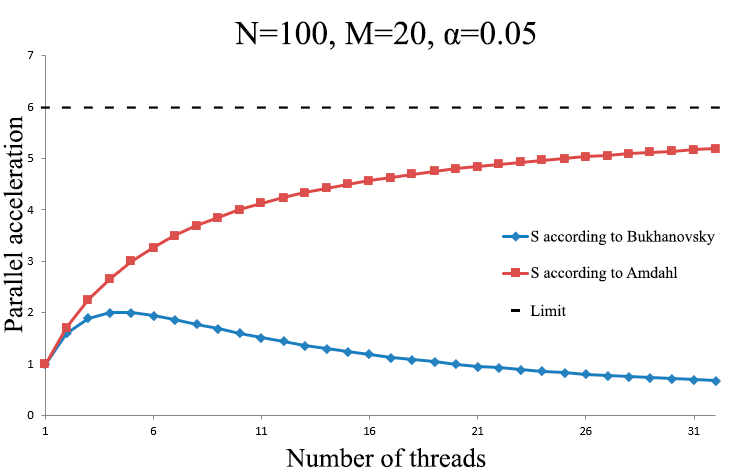
\includegraphics[width=1\linewidth]{GraphAmdalBuhunovsky}
		\caption{\textit{Graph of parallel acceleration versus number of threads}}
		\label{GraphAmdalBuhunovsky:image}
	\end{figure}
}
	{ %section2_5
	\subsection{Measuring the runtime of parallel programs}
	\par\textbf{Time measuring tools.} Measuring the runtime of a program in C is not a difficult problem, however, in parallel programming, a number of specific difficulties arise in performing this operation. Not all functions suitable for measuring the running time of a sequential program are suitable for measuring the running time of a multithreaded program.
	\par For example, if you use the ctime or localtime functions in a single-threaded program to measure the operating time of a section of code, they will successfully cope with the task. However, after parallelizing this part of the code, it is possible that hard-to-identify problems arise with incorrect time measurement, because both of these functions have an internal static variable, which, when trying to change it simultaneously by several threads, can take an unpredictable value.
	\par In order to solve the described problem, some C-compilers (for example, gcc) implemented thread-safe, re-entrant versions of these functions: ctime \textunderscore r and localtime \textunderscore r. Unfortunately, these functions are not available in all compilers. For example, in the Visual Studio compiler, a similar problem was solved using functions with completely different names and APIs: GetTickCount, GetLocalTime, GetSystemTime. For completeness, we list some other gcc functions that also allow you to measure time: time, getrusage, gmtime, gettimeofday.
	\par Another standard C-function clock also cannot be used to measure the execution time of multithreaded programs. However, the reason for this is not the lack of reenterability, but the features of the way this function calculates the elapsed time: clock returns the number of processor ticks that were executed when the program was running in total with all its threads. Obviously, this amount remains almost unchanged when the program executes with a different number of threads ("almost ', since the overhead costs of creating, deleting and managing threads are proposed to be considered insignificant in order to simplify the presentation).
	\par As a result, it turned out that a satisfactory \textit{cross-platform} solution for thread-safe time measurement with high accuracy (up to microseconds) by means of pure C language does not exist yet. However, the problem can be solved using third-party libraries, choosing those that have an implementation on the target platforms.
	\par The OpenMP system, which is implemented in the vast majority of modern compilers for all modern operating systems, stands out among such libraries. OpenMP has two functions for measuring time: omp\textunderscore get\textunderscore wtime и omp\textunderscore get\textunderscore wtick, which can be used in C-programs, if you include the omp.h header file and specify the necessary key during compilation (for example, in gcc this is the key ''-fopenmp'').
	\par\textbf{Time measurement error.} Another interesting point in measuring the running time of a parallel program is the method by which the researcher excludes various random errors from measurements that inevitably arise during an experiment in a running operating system, which can start the update or optimization process without notifying the user. The generally accepted is the way in which the researcher conducts not one, but immediately N experiments with a parallel program, without changing the initial data. It turns out N time measurements, which in the general case will be different due to various random factors affecting the experiment. Further, one of the following methods is most often used:
	\begin{enumerate}
		\item\textit{The calculation of the confidence interval:} consider all N measurements is calculated confidence interval, e.g., using Student's method.
		\item\textit{Search for the minimum measurement:} among N measurements, the smallest is chosen and it is used as the final result.
	\end{enumerate}
	\par The first method gives the correct result only if the measurement errors are distributed according to the normal law. This is most often the case, therefore, the application of the method is justified and allows you to get additional information about the possible use of the tested program in living conditions of a running OS.
	\par The second method does not impose requirements on the form of the law of distribution of measurement errors, and this compares favorably with the previous one. In addition, for large N, the choice of the minimum metering will make it possible to exclude from the experiment all the background influences of the operating system and to obtain as an result an accurate measurement of the operating time of the program under ideal conditions.
	\par\textbf{Practical example.} Let us compare by example the methods described above to get rid of the error of experimental time measurements. We will measure the OpenMP overhead for creating and deleting threads as follows:
	\begin{figure}[H]
		\lstinputlisting{OpenMPExampleTimeMeasurement.cpp}
	\end{figure}
	In line 3, we instruct OpenMP that when entering the parallel area located further in the program, i threads are created. If you do not give this indication, OpenMP will create the number of threads by the number of calculators available in the system (cores or logical processors). In line 4, we start the parallel program area, OpenMP creates i threads. In line 5, we give instructions to execute the following simple instruction in only one thread (the rest of the threads will not do any work. This is necessary so that only the costs of creating / deleting threads fall in the measured time of work, and all other costs would be lost against their background. The parallel area ends in line 6. OpenMP deletes the i number of  threads from the memory. A more detailed description of the OpenMP commands used can be found in section~\ref{OpenMP:section} \textit{''OpenMP Technology''} of this book.
	\par Experiments with this program were conducted on a computer with an Intel Core i5 processor (4 logical processors) with 8 gigabytes of RAM in the Debian Wheezy operating system. Empirically, it was revealed that the operating system used on an accessible hardware platform cannot create more than 381 threads in the OpenMP program (this explains the value in line 1). A total of $N = 100$ experiments were carried out, the results of which were processed by each of the two described methods. The results are shown in the figure.~\ref{OpenMPExpensesOnCreatingThreads:image}.
	\begin{figure}[H]
		\includegraphics[width=1\linewidth]{OpenMPExpensesOnCreatingThreads}
		\caption{\textit{OpenMP overhead measurement results for thread creation and deletion}}
		\label{OpenMPExpensesOnCreatingThreads:image}
	\end{figure} 
	\par The measured value (T2 - T1) in milliseconds is plotted along the ordinate axis, and the values of variable i, which indicate the number of created flows, are plotted on the abscissa axis. The upper graph, consisting of blue squares, shows the average value (T2 - T1) for the 100 experiments performed. The confidence interval is not shown, as it would clutter the graph without adding informativeness, but the width of the confidence interval with a confidence level of 90 \% approximately corresponds to the vertical spread of the squares of the upper graph for neighboring values of i.
	\par The lower graph, consisting of rhombs, represents the minimum of 100 measurements (T2 - T1) for the values of i indicated on the x-axis. We see that even a large number of experiments was not enough for the lower graph to have a smooth continuous structure without noticeable fluctuations.

}
}
	{ %section3
	\section{Practical Aspects of Parallel Programming}
	{ %section3_1
	\subsection{Debugging Parallel Programs}
	\par Parallel program debugging tools are built into most popular integrated development environments (IDEs), for example: Visual Studio, Eclipse CDT, Intel Parallel Studio, etc. These tools include convenient visualization of timing diagrams of thread execution, automatic search for suspicious program sections in which data races and deadlocks can be observed.
	\par Despite the effectiveness of existing debugging tools, there are significant difficulties when working in a debugger with a parallel program, because for its correct functioning, the debugger adds additional instructions to the machine code of the source parallel program that change the timing diagram of thread execution in relation to each other. This can lead to situations when during the testing of the program in the debugger there are no data races and deadlocks that will fully appear when the Release version of the program is launched.
	\par Also, during debugging of a multi-threaded program, it should be borne in mind that its behavior (both during regular operation and during debugging) can significantly differ when using a single-core and multi-core processor. When several threads are launched on a single-core machine, they will be executed in time-sharing mode, i.e. sequentially. This means that in this case many problems with shared access to memory and ensuring coherence of caches inherent in multi-core systems will not be observed. In addition, when debugging a program on a single-core system, a programmer can use implicit techniques to ensure the sequence of operations.
	\par For example, a programmer may incorrectly assume that when executing a high-priority thread, a low-priority thread cannot take over the processor. This assumption is correct only in a single-core system, because in the presence of several cores and a small number of high-priority threads, a situation may well be observed when a low-priority thread takes possession of one of the cores, while the high-priority thread is operating on the neighboring core.
	\par
}
	{ %section3_2
	\subsection{Memory Managers for Parallel Programs}
	\par When calling malloc / free functions in a single-threaded program, there are no problems even with a rather high call intensity of one of them. However, in parallel programs, these functions can become a bottleneck because when they are used simultaneously from several threads, a shared resource (memory management manager) is blocked, which can lead to a significant degradation in the speed of a multithreaded program.
	\par Despite the formal thread safety of standard memory functions, they can become thread-inefficient when the memory of several threads running in parallel is very intensive.
	\par To solve this problem, there are a number of third-party programs called the "Memory Management Manager (MUP)'' (Memory Allocator), both paid and free, open source. Each of them has its own advantages and disadvantages, which should be considered when choosing. We list the most common MUPs with links to official sites:
	\begin{itemize}
		\sloppy
		\item tcmalloc: \url{http://goog-perftools.sourceforge.net/doc/tcmalloc.html}
		\item ptmalloc: \url{http://www.malloc.de/malloc/ptmalloc3-current.tar.gz}
		\item dmalloc: \url{http://dmalloc.com/}
		\item HOARD: \url{http://www.hoard.org/}
		\item nedmalloc: \url{http://www.nedprod.com/programs/portable/nedmalloc/}
		\item jemalloc: \url{http://jemalloc.net/}
		\item mimalloc: \url{https://github.com/microsoft/mimalloc}
	\end{itemize}
	\par The listed MUPs are designed in such a way that they can 'silently' replace the standard MUP libraries of the C language C for the parallel program. This means that the choice of a particular MUP does not affect the source code of the program, so the general practice of using third-party MUPs is as follows: parallel program it is initially created using the libc MUP, then the profiling of the running program is performed, then when a bottleneck is detected in the malloc / free functions, a decision is made to replace the standard MUP with one of the listed.
	\par
	\par
}
	{ %section3_3
	\subsection{OpenMP Technology}
	\label{OpenMP:section}
	\par\textbf{Brief description of the technology.} The first version of the OpenMP standard appeared in 1997 with the support of the largest IT companies in the world (Intel, IBM, AMD, HP, Nvidia, etc.). The aim of the new standard was to offer a cross-platform parallelization tool that would be higher-level than the flow control APIs offered by the operating system. OpenMP is currently standardized for three programming languages: C, C ++ and Fortran.
	\par\textbf{Compiler support} The vast majority of existing modern C / C ++ compilers support OpenMP version 2.0 (for example, both gcc and Visual Studio). However, only a few compilers support the newer version of OpenMP 4.0, therefore, when setting forth the material, the OpenMP 2.0 technology will be used as the "common denominator"'.
	\par OpenMP defines a set of directives to the preprocessor, which instructs the compiler to replace the source code that follows them with a parallel version using tools available to the compiler, for example, POSIX Threads on Linux or Windows Threads on Microsoft operating systems. For correct translation of directives, you must specify a special key during compilation, the value of which depends on the compiler (examples are given in the table~\ref{compilerOpenMP:table}).
	\begin{table}[H]
		\caption{Compiler keys to run OpenMP}
		\label{compilerOpenMP:table}
		\begin{center}
			\begin{tabular}{|c|c|}
				\hline
				\textbf{Compiler name} & \specialcell{\textbf{Compiler Key} \\  \textbf{OpenMP}} \\
				\hline
				Gcc & -fopenmp \\
				\hline
				icc (Intel C/C++ compiler) & -openmp \\
				\hline
				Sun C/C++ compiler & -xopenmp \\
				\hline
				Visual Studio C/C++ compiler & /openmp \\
				\hline
				PGI (Nvidia C/C++ compiler) & -mp \\
				\hline
			\end{tabular}
		\end{center}
	\end{table}
	\par In addition to preprocessor directives, OpenMP defines a set of library functions. To call them in the source code, you need to include the OpenMP header file:
	\begin{figure}[H]
		\lstinputlisting{includeOpenMP.cpp}
	\end{figure}
	\par\textbf{Distinctive features.} Among other parallelization technologies, OpenMP stands out for the following important and characteristics:
	\begin{itemize}
		\item Incremental parallelization.
		\item Backward compatibility.
		\item High level of abstractions.
		\item Low coefficient of transformation.
		\item Support by the largest IT giants.
		\item Auto scaling.
	\end{itemize}
	\par\textit{Incremental parallelization.} OpenMP allows you to parallelize a sequential program using small iteration-edits, each of which will increase the parallelism coefficient of the program. This feature is unique because most other technologies suggest a significant change in the structure of the parallelized program at the first stage of the parallelization process, i.e. The first workable parallel version of the program appears after a long process of debugging and programming of new components, which are inevitably added during parallelization. OpenMP does not have this lack.
	\par\textit{Backward compatibility..} Most software technologies evolve with backward compatibility when a newer version of the program supports the functionality of old files. The term \textit{forward compatibility} has the opposite meaning: files created in the new version program remain functional when using the old version of the program. In the case of OpenMP, this means that the parallelized program will be correctly compiled in single-threaded mode even on an old compiler that does not support OpenMP. It is important to note that direct compatibility is ensured if, during parallelization, library functions of OpenMP are not used, and only preprocessor directives are present. If you have library functions, to ensure backward compatibility, you will need to write stub functions in the "omp.h'' file (some compilers can generate these stubs using a special key).
	\par\textit{High level of abstractions.} A single preprocessor OpenMP directive after processing by the compiler leads to a significant transformation of the source program with the addition of a large number of new logic, which is responsible for determining the number of processors available in the system, for starting and destroying threads, for distributing work between threads, etc. OpenMP takes care of all these operations; in return, the programmer receives a set of very high-level parallelization tools. High-level languages have a traditional drawback: in OpenMP there is no way to change some internal details of working with streams (for example, you cannot set the affinity of streams or reduce the overhead of creating / deleting streams).
	\par\textit{Low parallel transformation ratio (PTR)}. When parallelizing an existing sequential program, we need to make a fairly large number of changes to it. Let PTR be the ratio of the lines of the new program code that was added as a result of parallelization to the total number of lines of code in the program. In OpenMP, the CBT is usually significantly lower than most other parallelization technologies. This is due to the high level of abstraction of the OpenMP language (see the previous paragraph).
	\par\textit{Support by the largest IT giants.} Already during the development of OpenMP, it was supported by the largest players in the IT world. This ensured not only the high quality of standard development, but also the availability of off-the-shelf implementations of the standard in popular compilers. Despite the past twenty years, OpenMP has not lost its adherents and support for the latest versions with a fairly low delay appears in compilers. For example, with the current version of the OpenMP 4.5 standard, the most popular compilers already support OpenMP 4.0. The only exception is Microsoft. Their compiler for several versions invariably only supports OpenMP 2.0.
	\par\textit{Auto scaling.}  
	Low-level parallelization technologies (POSIX Threads, OpenCL) offer the programmer to manually control the number of threads created when performing parallel work. This provides the ability to flexibly manage and configure the process of creating threads depending on the number of processors (cores) available to the system, but it requires a large amount of non-automated work from the programmer. In OpenMP, scaling is controlled automatically, i.e. OpenMP itself asks the number of available processors from the operating system and selects the number of threads to create. But if necessary, OpenMP leaves the ability to set the required number of threads manually.
	\par\textbf{Examples of OpenMP programs.} Consider the simplest examples of running parallel programs below, starting with the traditional programming example "Hello, World ':
	\begin{figure}[H]
		\lstinputlisting{OpenMPExample1.cpp}
	\end{figure}
	\par The result of the work will be displayed several times in the console message. The number of messages is determined by the number of logical processors available to the system (for example, when using HyperThreading technology with two cores, the number of logical processors will be four). 
	\par The pragma directive extends to the next executable block. In this case, it is a call to the printf function, but one could enclose an arbitrary number of operations in curly braces to expand the executable block:
	\begin{figure}[H]
		\lstinputlisting{OpenMPExample2.cpp}
	\end{figure}
	In this program, a block of operations enclosed in braces is executed at the same time on several cores. At the same time, in line 5, the processor is instructed to perform the operation "i ++ '' atomically, i.e. not in parallel, but sequentially by each of the threads.
	\par On the one hand, this leads to the fact that the increment operation ceases to be parallelized, which reduces the speed of multi-core execution. On the other hand, the atomic directive is necessary in this case, because otherwise, a difficultly detectable problem with data race could arise, which manifests itself in a conflict when writing data to a common memory area simultaneously by several threads in the variable i. Note that the atomic directive can only be used for single-line simple assignment commands.
	\par o isolate more complex compound commands with the possible invocation of user and system functions, you should use the critical directive, which allows (unlike the atomic directive) the ability to expand its scope to a block of operations enclosed in curly braces, with each critical section having the name , allowing you to group different critical sections by this name to prevent the appearance of a single critical section distributed throughout the program:
	\begin{figure}[H]
		\lstinputlisting{OpenMPExample3.cpp}
	\end{figure}
	\par In this case, the printf function on line 4 is executed by all threads in parallel, which can lead to mixing of the output characters. On the contrary, the printf function in line 8 is executed by threads strictly in turn, which prevents possible conflicts between them, but slows down program execution due to the artificial limitation of the parallelism coefficient.
	\par An example of parallelizing a program containing a sequential call to the functions run \textunderscore function1 and run \textunderscore function2, which are independent of each other (i.e. do not use common data and the results of one do not affect the results of the other) and therefore allow convenient \textit{instruction parallelization} in pure form:
	\begin{figure}[H]
		\lstinputlisting{OpenMPExample4.cpp}
	\end{figure}
	\par Consider an example of loop parallelization using OpenMP. Suppose that in each cell of a one-dimensional array you need to write the index of this cell raised to the sixth power:
	\begin{figure}[H]
		\lstinputlisting{OpenMPExample5.cpp}
	\end{figure}
	\par Let the specified program run on a dual-core processor. Then the first processor calculates the values from a [0] to a [4], the second processor calculates the values from a [5] to a [9]. Apparently, when writing to the array, the processor does not interfere with each other, because work with different parts of the array. Let's try to optimize the previous option, reducing the number of multiplication operations for raising to the sixth power:
	\begin{figure}[H]
		\lstinputlisting{OpenMPExample6.cpp}
	\end{figure}
	\par In this case, the program will work correctly only if there is one processor (core). If there are several cores, the state of the data race will be observed while writing a new value to the tmp variable (line 4) by several threads, as a result, the array will be filled incorrectly. For example, suppose that the first thread performing iteration i = 2 wrote the number 8 in tmp. Now, when calculating a [2], the thread will try to write the number 8 * 8, however, if the second thread working with the iteration i = 7 has time to wedge before line 5, then the tmp value turns into 7 * 7 * 7, and the value of a [2] calculated by the first stream turns into $ 7 ^ 6 $, instead of the 64 ones. Lets correct the error as follows:
	\begin{figure}[H]
		\lstinputlisting{OpenMPExample7.cpp}
	\end{figure}
	\par A new element has appeared in the directive to the preprocessor: private. This element sets a comma-separated list of local (private) variables for each stream. In this case, there is only one such variable: tmp. Another equivalent way to correct the error is to transfer the declaration of the variable "int tmp '' inside the parallel region, which forces OpenMP to consider this variable local for each stream. The question may arise, why i was not added to the list of local variables. The answer is not obvious: by default, OpenMP considers the parallelized loop variable local.
	\par Any variable declared inside the parallel region is considered local in OpenMP, so such variables do not need to be specified in the list. Any variable declared outside this area is global (in our case, the global variable is a pointer to the array $a$). But if you need to explicitly indicate the globality of the variable, next to the private command, use the shared ($x$, \ldots) command, where $x$ defines the list of global variables.
	\par Consider an example in which you need to calculate the amount and for further execution to form an array of elements of the following series: $\{\;1^i,\;2^i,\;3^i,\;4^i,\;5^i\;\}$ for various values $i$, eg: $i\;=\;1,\;2,\;3$. Below is a solution to the problem, but intentionally make a mistake in it:
	\begin{figure}[H]
		\lstinputlisting{OpenMPExample8.cpp}
	\end{figure}
	\par In line 2, the parallel rsection starts, but the programmer forgets to indicate that the variables\textit{ j} and the tmp array must be local for each thread. Indeed, in line 4 there is an increment of the variable j common for the threads, which is executed by all threads simultaneously. In this situation, threads can interfere with each other by overwriting the value of\textit{ j.} We fix both errors as follows:
	\begin{figure}[H]
		\lstinputlisting{OpenMPExample9.cpp}
	\end{figure}
	\par We see that now the variable \textit{j} is explicitly defined as local (private). If we use the tmp array, the solution will be different - it can fit inside the parallel section (i.e. each stream will have its own instance of the tmp array independent of the others). Why can'twe just specify the tmp variable in the list of the private command, as was done for \textit{j}? The answer is related to the specifics of the C language: the \textit{tmp} variable is a pointer that does not change during the operation of the loop, but the contents of the memory pointed to by \textit{tmp }change. This means that specifying \textit{tmp} as a private variable would not solve the problem with data racing, because all streams would receive the same tmp address and interfere with each other, writing new values to this address.
	\par Let's consider one more error typical for parallel computing. The following program calculates the sum of numbers from 1 to 100:
	\begin{figure}[H]
		\lstinputlisting{OpenMPExample10.cpp}
	\end{figure}
	\par The \textit{sum} variable is global, so when you try to write a new value to it, the threads will interfere with each other. To fix the error, we have to use the local amount for each thread, and then we need to add all these local amounts:
	\begin{figure}[H]
		\lstinputlisting{OpenMPExample11.cpp}
	\end{figure}
	We see the beginning of the parallel area on line 2 -  at this point OpenMP creates several threads. In line 6, new threads are not created (because the parallel keyword is missing), but the threads entering the loop divide iterations among themselves, and do not complete each iteration as a whole. In line 8, the  thread calculating its partial amount tries to add this amount to the total amount. This has to be done using the atomic directive, which ensures that threads will not interfere with each other when overwriting sum.
	
	\par Another difficult point is the reinitialization of the variable \textit{sum} \textunderscore private on line 4: this is necessary because OpenMP does not initialize local variables, even if there are global variables with identical names. This solution is designed to reduce the overhead of copying variables.
	\par The described approach is working, but it is almost never used in practice, because the OpenMP standard for a whole class of similar tasks offers a higher-level and simpler solution. It consists in using the \textit{reduction} command:
	\begin{figure}[H]
		\lstinputlisting{OpenMPExample12.cpp}
	\end{figure}
	\par The \textit{reduction} command marks the listed variables as local, and at the end of the parallel region, all local variables are combined (aggregated) into one global variable with the same name using the specified operation. In our case, the operation is the amount. But OpenMP allows the use of '' * '', '' - '', '' / '' instead of the sign '' + ''. It is important that reduction, among other things, does not initialize the variables with the values of the original global variables, but with the most appropriate values of the aggregation logic: for example, when summing, the variable is initialized to zero, and when multiplying, it is initialized to one.
	\par When parallelizing a cycle, iterations may turn out to be unequal in the amount of work performed among themselves. This can lead to the fact that one thread will cope with the selected part of iterations much faster than the second thread and will be idle. To solve this problem, OpenMP offers four different ways to distribute iterations over threads. 
	\begin{itemize}
		\item\textit{Default method:} iterations are divided by the number of parts equal to the number of threads; each thread then performs its part and cannot take someone else's work.
		\item\textit{Static distribution:} iterations are divided into parts of the size specified by users; then, before starting work, each thread receives a fixed number of parts and performs only them without the ability to switch to others.
		\item\textit{Dynamic distribution:} iterations are divided into parts of the size specified by users; then the cycle starts immediately and each thread receives a new part of iterations as the work on the previous one is completed.
		\item\textit{Guided distribution:} the compiler divides the iterations into the number of parts equal to twice the number of threads; then the cycle starts immediately and each thread receives a new part of iterations as the work on the previous one is completed, while the size of the newly issued part decreases compared to the previous time, but cannot become less than the constant value specified by the user.
	\end{itemize}
	\par The user parameter mentioned in each method is called chunk \textunderscore size. Each of these methods has its own field of application in which it can provide maximum parallel acceleration. Note that the dynamic and guided modes, despite their logical nature, also have their drawbacks: they require significant overhead during the cycle compared to static. It is also important to understand that when choosing the number of chunk \ textunderscore size it is necessary to take into account the features of the caching mechanism.
	\par Consider an example of a static iteration distribution:
	\begin{figure}[H]
		\lstinputlisting{OpenMPExample13.cpp}
	\end{figure}
	\par With three cores, OpenMP will create three threads. The first thread will get iterations $i=1,\;4,\;7,\;…,\;97$ the second – iterations $i=2,\;5,\;8,\;…,\;98$, the third -  $i=3,\;6,\;9,\;…,\;99$. Note that choosing a small value for the parameter chunk \textunderscore size = 1 in this case does not have any negative effects. However, if i were used as an index when accessing the array, the proposed partitioning would lead to memory access not sequentially by sequential addresses, but sparse with step 3, which would degrade cache hit performance when using caching.
	\par Lets consider another example: 
	\begin{figure}[H]
		\lstinputlisting{OpenMPExample14.cpp}
	\end{figure}
	\par Here is an example of how you can tell OpenMP the number of threads to create using the num \textunderscore threads option (line 2), without focusing on the actually available number of cores (processors) on the computer. Next, the three created streams share 100 iterations among themselves in a way that is already familiar to us. However, the nowait option allows the first thread to cope with work not to wait for the others, but to proceed to the next work after the cycle. Behind a cycle in parallel, two functions are performed (lines 9 and 11). Each of the functions is enclosed in a section, which must have the parent element sections. As a result, the first thread freed up after the loop will calculate the function on line 9. The second freed thread will calculate the function on line 11. The third thread will not get work beyond its share of iterations in the first loop.
OpenMP's general requirement for parallelized loops is their \textit {canonicity}. A for loop is called \textit {canonical} if you can calculate the number of upcoming iterations in advance at its start. This is possible if the following conditions are met simultaneously:
	\begin{itemize}
		\item there are no break and return operations inside the loop;
		\item there is no goto operation inside the loop leading outside the loop;
		\item the loop variable (iterator) does not change inside the loop;
	\end{itemize}
In this case, the record of the cycle should have the form "for (i = A; i <B; i + = C)'', where the numbers A, B, C should not change during the operation of the cycle. The second parameter of the loop can use not only the sign '' <'', but also ''> '', ''> = '', '' <= ''. The third parameter of the loop can not only increment, but also decrement the loop variable (a short form of the entry `` i ++ '' is allowed).
	\par f iteration \textit{k} affects the results of iteration \textit{m}, then the cycle cannot be parallelized, because it is impossible to predict in advance the order of completion of iterations by multiple threads. The responsibility for detecting such conflicts lies with the programmer. For example, OpenMP will not detect the interdependence of iterations and compile the following program:
	\begin{figure}[H]
		\lstinputlisting{OpenMPExample15.cpp}
	\end{figure}
	\par In this program stream 0 most likely will not have time to fill in the element a [9] by the time when stream 1 will calculate the value a [10] = 2 * a [9].
	\par
}
	{ %section3_4
	\subsection{OpenCL Technology}
	\label{OpenCL:section}
	\par\textbf{Brief description of the technology.} OpenCL is a framework for writing computer programs related to parallel computing on various graphic and central processors, as well as FPGA. OpenCL includes a programming language that is based on the C99 language standard, and an application programming interface. OpenCL provides concurrency at the instruction level and data level and is an implementation of the GPGPU technique. OpenCL is a fully open standard, its use is not subject to licensing fees. Using this technology, heterogeneous parallel computing can be performed (distribute tasks between different devices).
	\par As we already know, it is possible to parallelize a program by tasks between a small number of productive cores (processors of modern PCs) or by data between thousands of simple slow cores (computing cores of modern GPUs). It is for problems solved using data parallelization that OpenCL is used.
	\par\textbf{OpenCL Technology Architecture} OpenCL divides two types of devices: \textit{host}, which controls the common logic, and \ textit{device}, which perform the calculations. The \textit{host} is usually the central processor, while the \textit{device} is the GPU and other devices. \textit{Device} divided into compute modules \textit{computer units}, which in turn consist of processing elements (\textit{processing elements}) (figure ~\ref{OpenCLArchitecture:image}). Direct calculations are performed in the processing elements of the device.
	\begin{figure}[H]
		\includegraphics[width=1\linewidth]{OpenCLArchitecture}
		\caption{\textit{OpenCL Architecture}}
		\label{OpenCLArchitecture:image}
	\end{figure}
	\par Physically\textit{computer unit} is \textit{work-group}, which consists of cells\textit{work-item}, which perform the calculations (figure~\ref{OpenCLWorkGroup:image}).
	\begin{figure}[H]
		\includegraphics[width=1\linewidth]{OpenCLWorkGroup}
		\caption{\textit{OpenCL  Architecture - the structure of work-group element}}
		\label{OpenCLWorkGroup:image}
	\end{figure}
	\par Commands in OpenCL form a queue. \textit {Host} routes commands to devices. These teams queue up similar teams. You can implement a queue in order and without compliance.
ID functions \textit{work-group} and \textit{work-item} are shown on  figure ~\ref{OpenCLWorkGroupItemExample:image}.
	\begin{figure}[H]
		\includegraphics[width=1\linewidth]{OpenCLWorkGroupItemExample}
		\caption{\textit{OpenCL. Work with  work-group и work-item}}
		\label{OpenCLWorkGroupItemExample:image}
	\end{figure}
	\par\textbf{Types of memory in OpenCL devices.} To interact with data, the programmer can use different levels of memory. On the figure ~\ref{OpenCLMemory:image} it we can see that the following types of memory exist:
	\begin{itemize}
		\item Private memory. The fastest of all kinds. Exclusive for every item of work.
		\item Local memory. It can be used by the compiler with a large number of local variables in any function. In terms of speed characteristics, local memory is much slower than register memory. Access from work items in one work-group.
		\item Constant memory. Fast enough of the available GPUs. It is possible to write data from the host, but at the same time, it is only possible to read data within the entire GPU. Dynamic allocation, unlike global memory, is not supported in constant memory.
		\item Global memory. The slowest type of memory available from the GPU. Global variables can be selected using the specifier, as well as dynamically. The global memory is mainly used to store large amounts of data received on the device from the host’s. In algorithms requiring high performance, the number of operations with global memory must be minimized.
	\end{itemize}	
	\begin{figure}[H]
		\includegraphics[width=1\linewidth]{OpenCLMemory}
		\caption{\textit{Types of memory in OpenCL devices}}
		\label{OpenCLMemory:image}
	\end{figure}
	The programmer must explicitly give copies between different memory.
		\par An OpenCL program may include the following sequence of actions:
		\begin{enumerate}
			\item\textbf{Platform choice:} clGetPlatformIDs, clGetPlatformInfo
			\item\textbf{Device choice:} clGetDeviceIDs, clGetDeviceInfo
			\item\textbf{Creating Computational Context:} clCreateContextFromType
			\item\textbf{Create a command queue:} clCreateCommandQueueWithProperties
			\item\textbf{Buffer Allocation:} clCreateBuffer
			\item\textbf{Creating a program object:} clCreateProgramWithSource
			\item\textbf{Code compilation:} clBuildProgram
			\item\textbf{Kernel Creation:} clCreateKernel
			\item\textbf{Working with Work-Group:} clGetKernelWorkGroupInfo 
			\item\textbf{Kernel execution:} clEnqueueNDRangeKernel 
			\item\textbf{Kernel Pending:} clWaitForEvents 
			\item\textbf{Profiling:} clGetEventProfilingInfo
		\end{enumerate}
Next, we consider some of these actions in more detail.
	\par\textbf{Platform, device, and context selection.}  \textit{(Context)} is required to manage OpenCL objects and resources. All OpenCL resources are context bound. The following data is associated with the context. (figure ~\ref{OpenCLContext:image}):
		\begin{itemize}
		\item devices
		\item object objects
		\item kernel
		\item memory objects
		\item command queues.
		\end{itemize}
	\begin{figure}[H]
		\includegraphics[width=1\linewidth]{OpenCLContext}
		\caption{\textit{OpenCL Architecture - Context}}
		\label{OpenCLContext:image}
	\end{figure}
It is possible to obtain information about the platform and the computing core using special functions, then to create a context:
		\begin{itemize}
			\item\textit{clGetPlatformInfo()} - contains information about the platform on which the program runs
			\item\textit{clGetDeviceDs()} - contains information about connected devices
			\item\textit{clGetDeviceInfo()} - contains information about this device: its type, compatibility, etc.
		\end{itemize}
Context can be created using the function \textit{clCreateContext()}. Here is an example of its creation:
	\begin{figure}[H]
		\includegraphics[width=1\linewidth]{OpenCLContextExample}
		\caption{\textit{OpenCL Architecture - Creating a context}}
		\label{OpenCLContextExample:image}
	\end{figure}
In line 3 we get the platform ID, in line 7 the ID of the first GPU on this platform, in line 11 we create a context for this device. You can read more about the arguments accepted by these functions in the documentation. There is also a function \textit{clCreateContextFromType()} to create the context associated with devices of a particular type.
	\par\textbf{Kernel.} A kernel is a function that is part of a program and runs in parallel on a device. The kernel is an analog of a stream function. The part running on the device consists of a set of cores declared with a qualifier \textbf{\textunderscore \textunderscore kernel}. Kernel compilation can be performed at runtime using API functions. Work within the same work group is performed simultaneously by all work items.
	\par When writing the kernel, you can use the following qualifiers for variables:
		\begin{itemize}
			\item\textunderscore \textunderscore global or global – data in global memory.
			\item\textunderscore \textunderscore constant or constant – data in constant memory.
			\item\textunderscore \textunderscore local or local – data in local memory.
			\item\textunderscore \textunderscore private or private – data in private memory.
			\item\textunderscore \textunderscore read\textunderscore only и \textunderscore \textunderscore write\textunderscore only – access mode qualifiers.
		\end{itemize}
	\par We can compile kernel code using functions \\ \textit{clCreateProgramWithSource()}, \textit{clBuildProgram()} и \textit{clCreateKernel()}. An example of compiling and running a program to multiply two arrays is given in figure~\ref{OpenCLKernelExample:image}.
	\begin{figure}[H]
		\includegraphics[width=1\linewidth]{OpenCLKernelExample}
		\caption{\textit{OpenCL - compiling and running the kernel}}
		\label{OpenCLKernelExample:image}
	\end{figure}
	\sloppy You can read more about other features of OpenCL technology %%on the resource \url{http://docplayer.ru/37490743-Programmirovanie-na-opencl.html} and %%
	in official documentation.
	\begin{enumerate}
		\sloppy
		\item OpenCL – official site:\url{http://www.khronos.org/opencl/}
		\item Intel OpenCL: \url{http://software.intel.com/en-us/articles/intel-opencl-sdk/}
		\item NVIDIA OpenCL: \url{https://developer.nvidia.com/cuda-zone}
		\item AMD OpenCL: \url{http://www.amd.com/us/products/technologies/stream-technology/opencl/Pages/opencl.aspx}
	\end{enumerate}
}
	{ %section3_5
	\subsection{Errors in multithreaded applications}
	\par In addition to the errors common to a programmer, there are a number of errors specific to parallel computing. These errors are caused by the following features of parallel programs:
	\begin{itemize}
		\item\textbf{Thread synchronization.} The programmer must ensure the correct sequence of operations performed by different flows. In the general case, it is impossible to say exactly in what sequence the flow commands will be executed, since the operating system may suspend the flow at any time.
		\item\textbf{Thread interaction.} Also, the programmer should not allow conflicts when accessing memory areas common to threads.
		\item\textbf{Load balancing.} If in a parallelized program one of the threads does 99 \% of the work, then even on a 64-core system parallel acceleration is unlikely to exceed 1.01.
		\item\textbf{Scalability.} In the ideal case, a parallel program should equally well parallel the work performed on any available number of processors. However, this is not easy to achieve and this often leads to hard-to-detect errors.
	\end{itemize}
	\par Further, we consider in more detail the following incomplete list of typical errors that occur in parallel programs regardless of the parallelization technology used:
	\begin{itemize}
		\item Loss of precision in floating point operations.
		\item Deadlocks
		\item Race conditions.
		\item АВА problems.
		\item Inversion of priorities.
		\item Starvation.
		\item False Sharing.
	\end{itemize}
	\par\textbf{Loss of accuracy} If a parallel program is used for floating-point operations when working with variables located in the threads common memory, then each time the program is launched, a different result of material calculations may be obtained. This is because when several threads work at the same time, it is impossible to accurately predict in what order the operating system will provide the processor with these threads, because at any time, any thread can be temporarily suspended at the discretion of the OS. This in turn leads to an indefinite sequence of floating-point operations, the result of which, as you know, may depend on the order.
	\par Consider an example illustrating the above:
	\begin{figure}[H]
		\lstinputlisting{OpenMPExample16.cpp}
	\end{figure}
	\par The variable s sums up the results of real calculations with eight threads. The result is s = 14.393189. However, if only one thread executes the same program (for this you need to set the parameter num \textunderscore threads to 1 in line 3), the result will be different: s = 14.357357. The difference between the two values is approximately 0.25 \%.
	\par t turns out that a parallel program can give different results when launched on different platforms. This should be taken into account when verifying parallel programs using their single-threaded unparalleled analogues.
	\par\textbf{Deadlocks.} One of the commonly used synchronization primitives is a mutex, which allows several threads to consistently and sequentially execute critical areas of code located inside parallel sections of code. Critical sections slow down the program, because at each moment of time, only one thread can be inside the critical section. Using mutexes, for example, omp functions are implemented \textunderscore set\textunderscore lock and omp\textunderscore unset\textunderscore lock в OpenMP. When these functions frame a certain section of code, you can make a critical section from it, the entrance to which is controlled by a conditional program lock. In complex programs can use several locks. This can lead to the fact that two threads, capturing several locks, stop the execution of each other without any possibility to exit the state of waiting for each other. This situation is called deadlock.
	\par The simplest example of deadlock is the operation of two threads, the first of which captures lock 1, then lock 2, and the second first captures lock 2, then lock 1. As a result, deadlock occurs if the operations are performed in the following order:
	\begin{itemize}
\item thread1 captured lock 1;
\item thread2 captured lock 2;
\item thread1 endlessly waits for release of lock 2;
\item thread2 endlessly waits for release of lock 1.
	\end{itemize}
	\par One of the unpleasant aspects of the described situation is that far from always mutual blocking occurs when debugging a program, when it could be easily detected and fixed, because the probability of overlapping events in the right way can be very small. As a result, a program that is running and delivered to the customer may “freeze” at random times for allegedly unknown reasons. Consider an example of an artificially implemented deadlock in which you can calculate the likelihood of its occurrence upon repeated startup.
	\par In the program below, in line 7, a stream is created that captures castle1, castle2 in an infinite loop and increments the variable s, freeing both locks after that. In line 13, a stream is created, which also infinitely increments s, but captures the locks in a different order: castle2, castle1. Line 19 creates a thread that monitors the state of s, polling this variable every 10 ms. If the last thread detects that the variable s has stopped changing, it prints a message about the deadlock and the program terminates.
	\begin{figure}[H]
		\lstinputlisting{deadlockExample.cpp}
	\end{figure}
	\par The experiments with the above program were carried out on a computer with an Intel Core i5 processor (4 logical processors) with 8 gigabytes of RAM in the Debian Wheezy operating system. The program was run 10,000 times, and 10,000 values of the variable s were obtained at the time the deadlock occurred. The results of these measurements are shown in the Figure~\ref{GraphDeadlock:image} in the form of a histogram of the distribution density s.
	\par In the above figure, the right borders of the columns are marked on the abscissa. The last column contains all hits from 3000 to infinity. The average value of s in the described case turned out to be 2445, i.e. two threads manage to capture and release the locks in an obviously wrong dangerous order without a deadlock approximately 1222.5 times.
	\begin{figure}[H]
		\includegraphics[width=1\linewidth]{GraphDeadlock}
		\caption{\textit{Histogram of the distribution of the number of starts of parallel programs before deadlock occurs}}
		\label{GraphDeadlock:image}
	\end{figure}
	\par To correct the described error, you need to make the lock capture order the same in all threads. It is sometimes advised throughout the program to establish some general rule for locking locks, for example, you can lock locks in alphabetical order.
	\par In addition to the described situation with the wrong order of capture of mutexes, there are other reasons for deadlocks. For example, the reacquisition of the mutex (lock). An incorrectly written program may try to re-capture the lock it has already captured, without first releasing it. In this case, a repeated attempt to capture completely stops the flow. If the program logic requires re-capture of the mutex (for example, to organize recursion), you should use a special subspecies of locks: recursive mutexes.
	\par\textbf{Race conditions} - an error in a parallel program in which the result of the calculation depends on the order in which the code is executed (it may be different each time the parallel program is launched). For example, consider the following situation. One thread changes the value of a global variable. At this time, the second thread prints this value. If the second thread prints the value before the first one changes it, the program will execute correctly, however, if the code is executed later, the new value assigned in the first thread will be displayed.
	\begin{figure}[H]
		\lstinputlisting{raceConditionalExample1.cpp}
	\end{figure}
	\par This problem can happen even in programs in which multi-threaded programming is not used explicitly, but some shared resources are used. For example, if a program copies text from an input field to the clipboard and then text is immediately inserted into another field, then if it runs on a computer alone, it will always work correctly. However, if a program that also uses the clipboard runs at the same time, it can overwrite the value of the clipboard, even if the copy and paste commands are located strictly one after another. Using shared resources, even for a very short time, can cause errors.
	\par Such a manifestation was called the "heisenbug '' or "floating error ''. To avoid this situation, it is necessary to block the recording of the new variable value in the first thread until the second thread finishes work. For example, in OpenMP technology, this problem can be solved as follows (save the old value in another variable):
	\begin{figure}[H]
		\lstinputlisting{raceConditionalExample2.cpp}
	\end{figure}
	\par\textbf{ABA problem} - the problem is that the thread reading the same value twice “thinks” that the data has not changed. For example, the first thread assigned a variable the value \textit{A}. The second thread assigned it the value \textit{B}, and then again \textit{A}. When the first thread reads this variable again, it is equal to A, and it “thinks” that nothing has changed. A more practical example from programming: an address is stored in a variable that points to the beginning of the array. The second thread frees memory for the new array with the free function and creates it with the malloc function, which allocated memory in the same place, since this memory area is already free. When the first thread compares the values of the pointer to the array before and after, it sees that they are equal and decides that the array has not changed, although new data is already stored in its place. To solve this problem, you can store a sign that the array has been modified.
	\par\textbf{Priority inversion.} Imagine a situation where there are 3 threads with priorities: high, medium and low, and threads with high and low priority capture the general mutex. Let the low priority thread capture the mutex and begin execution, but the medium priority thread interrupt it. Now, if a thread with a high priority intercepts a priority and starts executing, it will wait for the mutex to be freed, but a thread with a low priority cannot release it, since a thread with a medium priority has replaced it. This problem is solved by assigning all threads the same priority for the duration of the mutex retention.
	\par\textbf{Starvation} occurs when a thread with a low priority is in a ready state for a long time and is idle. Such starvation is caused by a lack of processor time, there is also a starvation caused by the inability to work with data (ban on reading and / or writing). In modern operating systems, this problem is solved as follows: even if the thread has a very low priority, it is still called for execution after a certain amount of time. In your programs, you should intelligently divide tasks between threads so that a thread performing a more important and long task has a higher priority.
	\par\textbf{False sharing} -  situation that arises with systems that support memory (cache) coherence, in which extra (unnecessary programs at this point) operations are performed to transfer data between streams. \textit{Memory (Caches) Coherence} - a memory property in which when changing the value of a memory cell by one process, these changes become visible in other processes. Large resources are spent on organizing such memory, since each time the value changes in one thread, the others need to be notified. Consider the following example:
	\begin{figure}[H]
		\lstinputlisting{falseSharingExample.cpp}
	\end{figure}
	\par If you run the functions fprint \textunderscore a and fprint \textunderscore b in two different threads, then due to the constant synchronization of memory between the threads, the program will run slowly, since a and b are on the same cache line (usually 64 bytes). It would be more reasonable to parallelize each loop between threads (for example, using the preprocessor directive  \#pragma omp parallel for in OpenMP).
}
}
	{ %section4
	\section{Laboratory research \#1. «Automatic program parallelization»}
	{ %section4_1
	\subsection{Work sequence}
	\begin{enumerate}
		\item Install Linux and the GCC compiler version 4.7.2 or higher on a computer with a multi-core processor. If you cannot install Linux or you do not have a computer with a multi - core processor, you can perform laboratory research on a virtual machine.
		\item Write a console program in C completing task in article 4 (see below). The program cannot use library functions for sorting, performing matrix operations, or calculating statistical values. The program cannot use library functions that are not represented in standard stdio.h, stdlib.h, math.h, sys/time.h header files. You must run the task 50 times with different initial values of the random number generator (RNG). The structure of the program is approximately as follows:
			\begin{figure}[H]
				\lstinputlisting{lab1Example.cpp}
			\end{figure}
		\item Сompile the program without using automatic parallelization following the next command: /home/user/gcc -O3 -Wall -Werror -o lab1-seq lab1.c
		\item Compile the written program using the built-in GCC tool for automatic parallelization (Graphite) with the following command  “/home/user/gcc -O3 -Wall -Werror -floop-parallelize-all -ftree-parallelize-loops=K lab1.c -o lab1-par-K” (assign at least 4 different integer values to the variable K in turn and explain your choice).
		\item The result is one non-parallelized program and four or more parallelized programs.
		\item Close all application programs running on the operating system (including Winamp, uTorrent, browsers, and Skype) so that they do not affect the results of subsequent experiments.
		\itemЗапускать файл lab1-seq из командной строки, увеличивая значения N до значения N1, при котором время выполнения превысит 0.01 с. Подобным образом найти значение N=N2, при котором время выполнения превысит 2 с.
		\itemИспользуя найденные значения N1 и N2, выполнить следующие эксперименты (для автоматизации проведения экспериментов рекомендуется написать скрипт):
			\begin{itemize}
				\itemзапускать lab1-seq для значений \\$N\;=\;{N1,\;N1+\Delta,\;N1+2\Delta,\;N1+3\Delta,…,\;N2}$ и записывать получающиеся значения времени delta\textunderscore ms(N) в функцию $seq(N)$;
				\itemзапускать lab1-par-K для значений \\$N\;=\;{N1,\;N1+\Delta,\;N1+2\Delta,\;N1+3\Delta,…,\;N2}$ и записывать получающиеся значения времени delta\textunderscore ms(N) в функцию $par-K(N)$;
				\itemзначение $\Delta$ выбрать так: $\Delta\;=\;(N2\;-\;N1)/10$.
			\end{itemize}
		\itemНаписать отчёт о проделанной работе.
		\itemПодготовиться к устным вопросам на защите.
		\itemНайти вычислительную сложность алгоритма до и после распараллеливания, сравнить полученные результаты.
		\sloppy
		\item\textbf{Необязательное задание №1 (для получения оценки «четыре» и «пять»).} Провести аналогичные описанным эксперименты, используя вместо gcc компилятор Solaris Studio (или любой другой на своё усмотрение). При компиляции следует использовать следующие опции для автоматического распараллеливания: \verb+«solarisstudio -cc -O3 -xautopar -xloopinfo lab1.c»+.
 		\item\textbf{Необязательное задание №2 (для получения оценки «пять»).} Это задание выполняется только после выполнения предыдущего пункта. Провести аналогичные описанным эксперименты, используя вместо gcc компилятор Intel ICC (или любой другой на своё усмотрение). В ICC следует при компиляции использовать следующие опции для автоматического распараллеливания: \verb+«icc -parallel -par-report -par-threshold K -o lab1-icc-par-K lab1.c»+.
			\parЕсли ключ \verb+«-par-report»+ не работает в вашей версии компилятора, то желательно использовать более актуальный ключ \\\verb+«-qopt-report-phase=par»+.
	\end{enumerate}
	
}
	{ %section4_2
	\subsection{Structure of the report}
	\begin{enumerate}
		\item Front page with the title of the university, student's full name, and the title of the research.
		\item Table of the report contents (indicating the page number, etc.).
		\item Description of the task to be performed (take it from parts 1 and 4).
		\item Brief description of the processor, operating system, and GCC compiler used for experiments (official name, version/model number, bit depth, number of cores, RAM capacity, etc.).
		\item Listing of the lab1.c program as a separate file.
		\item Tables of values and graphs of functions seq(N), par-K(N) indicating the value of parallel acceleration.
		\item Detailed conclusions with an analysis of the graphs and the results obtained.
		\item The report must be provided in paper or on a flash drive.
	\end{enumerate}
}
	{ %section4_3
	\subsection{Be ready to know/explain}
	\begin{enumerate}
		\item Each line of the program presented in the report.
		\item Purpose and main features of GCC, as well as the meaning of all the GCC compilation keys used in the research.
		\item Know the contents of lecture \#1.
		\item Please, take all the necessary files to demonstrate the working program with you.
	\end{enumerate}
}
	{ %section4_4
	\subsection{Task variants}
	\par The task variants are selected in accordance with the following description of the stages, given that the number A = LN*FN*SN, where LN, FN, and SN mean the number of letters in the last name, first name and second name of the student. You select the variant number in the corresponding tables by the formula X = 1 + ((A mod 47) mod B), where В is the number of elements in the corresponding table, and the mod operation means the remainder of the division. For example, if А = 476 and В = 5, we get \textbf{Х = 1 + ((470+6) mod 47) mod 5) = 1 + (6 mod 5) = 2}. The order of calculation must be as follows:
	\begin{enumerate}
		\item\textbf{Generate Stage.} Form an array M1 of dimension N, filling it with the function rand\textunderscore r (you cannot use rand) with random real numbers that have a uniform law in the range from 1 to A inclusively. Similarly, form an array of M2 of dimension N / 2 with random real numbers in the range from A to 10*A.
		\item\textbf{Map Stage.} Apply an operation from the table to each element in the M1 array:
			\begin{center}
				\begin{tabular}{|c|c|}
					\hline
					\specialcell{\textbf{Number of}\\ \textbf{the variant}} & \textbf{Operation} \\
					\hline
					1 & \specialcell{Hyperbolic sine with squaring} \\
					\hline
					2 & \specialcell{Hyperbolic cosine with an\\ increase by 1} \\
					\hline
					3 & \specialcell{Hyperbolic tangent with the\\ decrease by 1} \\
					\hline
					4 & \specialcell{Hyperbolic cotangent of\\ number's root} \\
					\hline
					5 & \specialcell{Division by $\pi$ with the raising\\ to the third power} \\
					\hline
					6 & \specialcell{Cubic root after division by e} \\
					\hline
					7 & \specialcell{Square root exponent\\ (i.e. M1[i] = exp(sqrt(M1[i])))} \\
					\hline
				\end{tabular}
			\end{center}
			Then, in the M2 array, add each element in turn with the previous one (you will need a copy of the M2 array, from which you will need to take operands for this), and apply an operation from the table to the result of the addition (assume that for the initial element of the array, the previous element is zero):
			\begin{center}
				\begin{tabular}{|c|c|}
					\hline
					\specialcell{\textbf{Number of}\\ \textbf{the variant}} & \textbf{Operation} \\
					\hline
					1 & Sine modulus (i.e. M2[i] = |sin(M2[i] + M2[i-1])|) \\
					\hline
					2 & Cosine modulus \\
					\hline
					3 & Tangent modulus \\
					\hline
					4 & Cotangent modulus \\
					\hline
					5 & Natural logarithm of the tangent modulus \\
					\hline
					6 & Decimal logarithm raised to the e power \\
					\hline
					7 & Cubic root after multiplying by $\pi$ \\
					\hline
					8 & Square root after multiplying by e \\
					\hline
				\end{tabular}
			\end{center}
		\item\textbf{Merge Stage.} In arrays M1 and M2 apply the operation from the table to all elements in pairs with the same indexes in (write the result in M2): 
			\begin{center}
				\begin{tabular}{|c|c|}
					\hline
					\specialcell{\textbf{Number of}\\ \textbf{the variant}} & \textbf{Operation} \\
					\hline
					1 & Raising to a power (i.e. M2[i] = M1[i]\verb+^+M2[i]) \\
					\hline
					2 & Division (i.e. M2[i] = M1[i]/M2[i]) \\
					\hline
					3 & Multiplication \\
					\hline
					4 & Selecting the larger (i.e. M2[i] = max(M1[i],M2[i]))) \\
					\hline
					5 & Selecting the smaller \\
					\hline
					6 & Absolute difference \\
					\hline
				\end{tabular}
			\end{center}
		\item\textbf{Sort Stage.} The resulting array must be sorted by the method specified in the table (you cannot use library functions for this; you can take the implementation as freely available source code):
			\begin{center}
				\begin{tabular}{|c|c|}
					\hline
					\specialcell{\textbf{Number of}\\ \textbf{the variant}} & \textbf{Operation} \\
					\hline
					1 & Selection sort \\
					\hline
					2 & Comb sort \\
					\hline
					3 & Heapsort \\
					\hline
					4 & Stupid sort \\
					\hline
					5 & Gnome sort\\
					\hline
					6 & Insertion sort \\
					\hline
					7 & Selection sort \\
					\hline
				\end{tabular}
			\end{center}
		\item\textbf{Reduce Stage.} Calculate the sine sum of those array M2 elements, which give an even number when divided by the minimum non-zero element of the mass M2 (when determining parity, count only the integer part of the number). The result of the program at the end of the fifth stage must be a single number X, which should be used for verification of the program after making changes to it (for example, before and after parallelization, the final number X  should not change within the margin of error). The value of the number X should be reported for different values of N.
		\par
	\end{enumerate}
}
}

	{ %section5
	\section{Laboratory research \#2. "Study of the parallel libraries for C-programs effectiveness"{}}
	{ %section5_1
	\subsection{Work sequence}
	\begin{enumerate}
		\item In the source code of the program obtained as a result of laboratory research \#1, replace all loops with calls of mathematical functions at the Map and Merge stages with vector analogs from the «AMD Framewave» library (\url{http://framewave.sourceforge.net}). Make sure that a specific Framewave function is marked as MT (Multi-Threaded), i.e. parallelized, when selecting it. The full list of available functions can be found here: \url{http://framewave.sourceforge.net/Manual/fw_section_060.html#fw_section_060}. For example, the Framewave function min has only SSE2 in the list of supported technologies, but not MT. 
			\par\textit{Note:} the choice of the Framewave library is not mandatory, you can use any other parallel library, if it has the necessary functions parallelized. For example, you can use ATLAS (you need to learn trottling and energy saving for this library, as well as to deal with the mechanism of changing the number of threads) or Intel Integrated Performance Primitives.
		\item Add a call to the Framewave function \\SetNumThreads(M) to the beginning of the program to set the number of threads created by the parallel library that are used when executing parallel Framewave functions. Set number M from the command-line parameter (argv) for ease of experiments automatization.
		\item Compile the program without using the automatic parallelization options used in laboratory research \#1. Conduct the experiments with the resulting program for the same values $N_1$ and $N_2$, which were used in laboratory research \#1, at $M\;=\;1,\;2,\;…,\;K$, where $K$ is the number of processors (cores) on the experimental stand.
		\item Compare the obtained results with the results of laboratory research #1: show how the program execution time, parallel acceleration, and parallel efficiency have changed on the graphs.
		\item Write a report on the work performed.
		\item Be ready to answer questions on the presentation.
		\item\textbf{Optional task \#1} (to get good and highest mark). Investigate parallel acceleration for different values of $M > K$, i.e. estimate virtualization overhead when creating a large number of threads. Give a graph of the processor (cores) loading during the execution of the program at $N\;=\;N_2$ for all used $M$. to illustrate that the program is really parallelized. You can write a script or just make a screenshot of the Task Manager, specifying the start and the end points of the experiment on the screenshot to get a graph (you need to give the text of the script or the name of the used Manager in the report).
		\item\textbf{Optional task \#2} (to get excellent mark). You should perform this task only after the previous task has been completed. Calculate the parallelization coefficient for all experiments and plot it on graphs using Amdahl's law. Explain the results.
	\end{enumerate}
}
	{ %section5_2
	\subsection{Structure of the report}
	\begin{enumerate}
		\item Front page with the title of the university, student's full name, and the title of the research.
		\item Table of the report contents (indicating the page number, etc.).
		\item Brief description of the processor, operating system, and GCC compiler used for experiments (official name, version/model number, bit depth, number of cores, RAM capacity, etc.).
		\item Description of the parallel library configuration features, including the description of the steps sequence taken to install the library and the configuration options used.
		\item Full text of the resulting parallel program, as well as the text of all the scripts used to compile the program and conduct experiments.
		\item Graphs of program execution time functions, as well as graphs of parallel acceleration and parallel efficiency for different  $N$ and $M$ (you may combine several graphs in the same coordinate system).
		\item Detailed conclusions with an analysis of the graphs and the results obtained. The report mist be provided in paper or on a flash drive.
	\end{enumerate}
}
	{ %section5_3
	\subsection{Be ready to know/explain}
	\begin{enumerate}
		\item Each line of the program presented in the report.
		\item The purpose of all the compilation keys used in the research.
		\item Know the contents of lecture \#2.
		\item Please, take all the necessary files to demonstrate the working program with you.
	\end{enumerate}
}
}

	{ %section6
	\section{Laboratory research \#3. «Loop parallelization using OpenMP technology»}
	{ %section6_1
	\subsection{Work sequence}
	\begin{enumerate}
		\item Add the following OpenMP Directive to all for-loops in the program from Laboratory research \#1: \\	
''\#pragma omp parallel for default(none) private(...) shared(...)''. The presence of all the listed parameters in the specified directive is mandatory.
		\item Check all for-loops for internal dependencies on data between iterations. If dependencies are found, use the directive ''\#pragma omp critical'' or ''\#pragma omp atomic'' (if the operation is atomic), or the reduction parameter (preferably), or refuse to parallelize the loop at all (your choice must be justified) to protect critical sections.
		\item Make sure that the resulting program has the property of direct compatibility with compilers that do not support OpenMP (you can compile the program without the option ''–fopenmp'' to check this. As a result, there should be no error messages, and the program should work correctly).
		\item Conduct experiments by measuring the parallel acceleration. Compare parallel acceleration graphs with Laboratory research \#1 and \#2.
		\item Conduct the experiments by adding the ''schedule'' parameter and varying the schedule type in the experiments. You need to do the research for all possible schedules: static, dynamic, guided. You can choose the method of varying the chunk\textunderscore size parameter yourself (but there must be at least 5 points of variation). Compare the parallel acceleration for different schedules with the results of article 4.
		\item Choose the best option for different $N$ from those discussed in article 4 and 5. Formulate the conditions under which best results would be obtained by using other types of writing.
		\item Find the computational complexity of the algorithm before and after parallelization and compare the results obtained.
		\item Write a report on the work performed.
		\item Be ready to answer questions on the presentation.
		\item\textbf{Optional task \#1} (to get good and excellent mark). Give a graph of the CPU load (cores) from the time when the program is running at $N\;=\;N_1$ for the best parallelization option to illustrate that the program is really parallelized. You can write a script or just make a screenshot of the Task Manager, specifying the start and the end points of the experiment on the screenshot to get a graph (you need to give the text of the script or the name of the used Manager in the report). You need to provide a graph of the load changes over the entire time of the program execution, because providing a single instant load measurement by the htop utility is not enough.
		\item\textbf{Optional task \#2} (to get excellent mark). Build a parallel acceleration graph for points $N\;<\;N_1$ and find the values of $N$at which the overhead of parallelization exceeds the gain from parallelization (independently for different types of schedules).
	\end{enumerate}
}
	{ %section6_2
	\subsection{Structure of the report}
	\begin{enumerate}
		\item Front page with the title of the university, student's full name, and the title of the research.
		\item Table of the report contents (indicating the page number, etc.).
		\item Brief description of the task to be completed.
		\item Characteristics of the processor, operating system and GCC compiler used for the experiments (exact name, version/model number, bit depth, number of cores, etc.).
		\item Listing of the program using the schedule parameter.
		\item Detailed conclusions with an analysis of each of the graphs.
		\item The report is provided in soft or hard copy including the listing of the program. Be ready to compile and run this file on the computer in the classroom (or your laptop) at the request of the teacher.
	\end{enumerate}
}
	{ %section6_3
	\subsection{Be ready to know/explain}
	\begin{enumerate}
		\item Each line of the program presented in the report.
		\item Conclusions obtained as a result of the work.
		\item Objectives of each OpenMP Directive used in the program.
		\item Repeat the contents of lecture \#3, read the "OpenMP Technology" Chapter in the guidance manual
		\item Read the article about the \#pragma\textunderscore omp\textunderscore for Directive in the book "Parallel programming using OpenMP technology: Study guide" by A. S. Antonov and know the answers to the questions at the end of the corresponding chapter.
	\end{enumerate}
}
}

	{ %section7
	\section{Laboratory research \#4. «The method of confidence intervals for measuring the execution time of a parallel OpenMP program»}
	{ %section7_1
	\subsection{Work sequence}
	\begin{enumerate}
		\item1.	In the program resulting from the execution of Laboratory research~\#3, change the Generate stage so that the generated set of random numbers does not depend on the number of threads running the program. For example, before calling \texttt{rand\textunderscore r},  at each iteration of $i$, you can call the \texttt{srand(f(i))} function, where \texttt{f} is an arbitrary function. You can think of and use any other method.
		\item Replace the gettimeofday function calls to \texttt{omp\textunderscore get\textunderscore wtime}.
		\item Parallelize the calculations at the Sort stage, for which you can perform sorting in two stages:
			\begin{itemize}
				\item Sort the first and the second half of the array in two independent threads (you can use the OpenMP Directive ''parallel sections''); 
				\item Combine the sorted halves into a single array.
			\end{itemize}
		\item Write a function that outputs a message to the console about the current percentage of program shutdown once a second. Run the specified function in a separate thread running in parallel with the main computing cycle.
		\item Ensure forward compatibility of a written parallel program. To do this, conditionally redefine all called functions of the form «\texttt{omp\textunderscore *}» in preprocessor directives, for example:
			\begin{figure}[H]
				\lstinputlisting{lab4Example.cpp}
			\end{figure}
		\item Conduct the experiments with the resulting program, varying $N$ from $min(\frac{N_x}{2},\;N_1)$ to $N_2$, for the same values $N_1$ and $N_2$, which were used in laboratory research \#1, where $N_x$ is the number of $N$, in which the overhead of parallelization exceeds the gain from parallelization. Write a report on the work performed. Be ready to answer questions on the presentation.
		\item\textbf{Optional task (to get good and excellent mark).} Reduce the number of iterations of the main loop from 100 to 10 and perform experiments by measuring the execution time using the following methods:
			\begin{itemize}
				\item Use the minimum measurement of ten received ones; 
				\item Calculate the confidence interval with a confidence level of 95\% based on ten dimensions.
			\end{itemize}
			Give graphs of parallel acceleration for both methods in the same coordinate system, furthermore, giving the lower and upper bounds of the confidence interval by two independent graphs is advisable.
		\item\textbf{Optional task (to get highest mark):} in part 3 at the Sort stage, perform parallel sorting of $k$ parts of the array (not two parts) in $k$ threads, where $k$ is the number of processors (cores) in the system, which becomes known only at the program execution stage using the command \texttt{«k = omp\textunderscore get\textunderscore num\textunderscore procs()}».
	\end{enumerate}
}
	{ %section7_2
	\subsection{Structure of the report}
	\begin{enumerate}
		\item Front page with the title of the university, student's full name, and the title of the research.
		\item Table of the report contents (indicating the page number, etc.).
		\item Brief description of the task to be completed.
		\item Characteristics of the processor, operating system and GCC compiler used for the experiments (exact name, version/model number, bit depth, number of cores, etc.).
		\item Listing of the program, the scripts, and tools used in the process, indicating the launch parameters.
		\item Detailed conclusions with an analysis of each of the graphs.
	\end{enumerate}
	\par The report is provided in soft or hard copy together with the full text of the program. Be ready to compile and run this file on the computer in the classroom (or your laptop) at the request of the teacher.
	\par
}
	{ %section7_3
	\subsection{Be ready to know/explain}
	\begin{enumerate}
		\item Each line of the program presented in the report.
		\item Conclusions obtained as a result of the work.
		\item Objectives of each OpenMP Directive used in the program.
		\item Repeat the contents of lecture \#4, read the "OpenMP Technology"\ Chapter in the guidance manual.
		\item Know the answers to questions from the "Task"\ sections of the "Parallel programming using OpenMP technology: Study guide"\ book by A. S. Antonov:  (see pages 12, 28, 35, 54).
		
	\end{enumerate}
}
}

%	{ %section8
	\section{Laboratory research \#5. "Parallel programming using the POSIX Threads standard"{}}
%переделать для других лаб
	{ %section8_1
	\subsection{Порядок выполнения работы}
	\begin{enumerate}
		\item Take OpenMP program from Laboratory research \#5, in which all the stages of calculation are parallelized, as an initial one. Make sure that this program correctly implements simultaneous access to the common variable used to output the program completion percentage to the console.
		\item Change the source code so that the "POSIX Threads" standard is used instead of OpenMP directives:
			\begin{itemize}
				\item change only one stage (Generate, Map, Merge, Sort), which is a bottleneck, as well as the output of the program completion percentage to the console function to get \textbf{satisfactory mark};
				\item change the entire program (you are allowed to use "schedule static" as the loops schedule) to get \textbf{good} and \textbf{excellent mark};
				\item parallelize at least one cycle by manually implementing "schedule dynamic" or "schedule guided" schedule to get \textbf{excellent mark}.
			\end{itemize}
		\item Conduct experiments and compare the results of two parallel programs ("OpenMP" and "POSIX Threads"). The comparison must describe the following aspects of both programs (for different $N$):
			\begin{itemize}
				\item total time for solving the task;
				\item parallel acceleration;
				\item the percentage of time spent at each stage of the calculation ("normalized chart with areas and accumulation");
				\item the number of code lines added during parallelization, as well as a rough estimate of the time spent on parallelization (programmer's overhead);
				\item other aspects that you have found out yourself (\textbf{Mandatory point});
			\end{itemize}
	\end{enumerate}
}
	{ %section8_2
	\subsection{Structure of the report}
	\begin{enumerate}
		\item Front page with the title of the university, student's full name, and the title of the research.
		\item Table of the report contents (indicating the page number, etc.).
		\item Brief description of the task to be completed.
		\item Characteristics of the processor, operating system and GCC compiler used for the experiments (exact name, version/model number, bit depth, number of cores, etc.).
		\item Listing of the programs ("OpenMP" and "POSIX Threads") and the scripts and the tools with the launch parameters used in the process.
		\item Detailed conclusions with an analysis of each of the graphs.
	\end{enumerate}
	\par The report is provided in soft or hard copy together with the full text of the program. Be ready to compile and run this file on the computer in the classroom (or your laptop) at the request of the teacher.
	\par
}
	{ %section8_3
	\subsection{Be ready to know/explain}
	\begin{enumerate}
		\item Each line of the program presented in the report.
		\item Conclusions obtained as a result of the work.
		\item Be ready to answer questions based on the contents of lecture \#5.
	\end{enumerate}
}
}

%	{ %section9
	\section{Laboratory research \#6. «Study of OpenCL Technology»}
	{ %section9_1
	\subsection{Work sequence}
	\begin{enumerate}
		\item Implement one (to get satisfactory mark) or two (to get good mark) stages of your program from previous laboratory research.  Perform calculations on the CPU or the GPU (at your discretion, but the GPU is preferable).
		\item\textbf{Optional task (to get excellent mark).}
			\begin{itemize}
				\item Complete tasks to get satisfactory and good mark.
				\item Calculate the confidence interval.
				\item Count time in 2 ways: using profiling and using usual metering (previous tasks).
				\item Evaluate the overhead.
				\item* Optional task for students with a lot of free time: Perform calculations together on the GPU and the CPU (i.e. iterations are divided in a certain proportion between the GPU and the CPU and performed simultaneously on them).
			\end{itemize}
		\item You may also write this laboratory research in CUDA.
	\end{enumerate}
}
	{ %section9_2
	\subsection{Structure of the report}
	\begin{enumerate}
		\item Front page with the title of the university, student's full name, and the title of the research.
		\item Table of the report contents (indicating the page number, etc.).
		\item Brief description of the task to be completed.
		\item Characteristics of the processor, operating system and GCC compiler used for the experiments (exact name, version/model number, bit depth, number of cores, etc.)
		\item Listing of the parallelized program (for articles 2 and 3).
		\item Detailed conclusions.
	\end{enumerate}
	\par The report is provided in soft or hard copy together with the full text of the program. Be ready to compile and run this file on the computer in the classroom (or your laptop) at the request of the teacher.
	\par
}
	{ %section8_3
	\subsection{Be ready to know/explain}
	\begin{enumerate}
		\item Each line of the program presented in the report.
		\item Conclusions obtained as a result of the work.
		\item Read the~\ref{OpenCL:section} \textit{OpenCL Technology} Chapter in the guidance manual.
		\item Study the contents of the lecture on OpenCL technology.
	\end{enumerate}
}
}

%	{ %bibliography
	\phantomsection
	\section*{References}
	\addcontentsline{toc}{section}{References}
	\begin{enumerate}
		\sloppy
		\itemСоснин В.В., Балакшин П.В. Введение в параллельные вычисления. – СПб: Университет ИТМО, 2016. – 51 с.
		\item Top 500 supercomputers list. URL: \href{https://www.top500.org/} {https://www.top500.org/} (дата обращения: 12.02.19).
		\itemВикипедия. Симметричная мультипроцессорность. URL: \href{https://ru.wikipedia.org/wiki/%D0%A1%D0%B8%D0%BC%D0%BC%D0%B5%D1%82%D1%80%D0%B8%D1%87%D0%BD%D0%B0%D1%8F_%D0%BC%D0%BD%D0%BE%D0%B3%D0%BE%D0%BF%D1%80%D0%BE%D1%86%D0%B5%D1%81%D1%81%D0%BE%D1%80%D0%BD%D0%BE%D1%81%D1%82%D1%8C}{https://ru.wikipedia.org/wiki/Симметричная\_многопроцессорность} (дата обращения: 12.02.19).
		\itemВикипедия. Массово-параллельная архитектура. URL: \href{https://ru.wikipedia.org/wiki/%D0%9C%D0%B0%D1%81%D1%81%D0%BE%D0%B2%D0%BE-%D0%BF%D0%B0%D1%80%D0%B0%D0%BB%D0%BB%D0%B5%D0%BB%D1%8C%D0%BD%D0%B0%D1%8F_%D0%B0%D1%80%D1%85%D0%B8%D1%82%D0%B5%D0%BA%D1%82%D1%83%D1%80%D0%B0}{https://ru.wikipedia.org/wiki/Массово-параллельная архитектура} (дата обращения: 12.02.19).
		\itemВикипедия. OpenCL. URL: \href{https://ru.wikipedia.org/wiki/OpenCL}{https://ru.wikipedia.org/wiki/OpenCL} (дата обращения: 13.02.19).
		\itemВведение в GPU-вычисления - CUDA/OpenCL. URL: \href{http://my-it-notes.com/2013/06/gpu-processing-intro-cuda-opencl/}{http://my-it-notes.com/2013/06/gpu-processing-intro-cuda-opencl/} (дата обращения: 13.02.19).
		\itemБастраков С.И. Программирование на OpenCL. - Нижний новгород: ННГУ, 2011.
		\item OpenCL – официальный сайт URL: \href{http://www.khronos.org/opencl/}{http://www.khronos.org/opencl/} (дата обращения: 13.02.19).
		\itemАнтонов А.С. Параллельное программирование с использованием технологии MPI. - Москва: МГУ, 2004. - 72 с.
		\itemАнтонов А.С. Параллельное программирование с использованием технологии OpenMP. - Москва: МГУ, 2009.- 78 с.
		\itemВикипедия. Параллельные вычисления. URL: \href{https://ru.wikipedia.org/wiki/%D0%9F%D0%B0%D1%80%D0%B0%D0%BB%D0%BB%D0%B5%D0%BB%D1%8C%D0%BD%D1%8B%D0%B5_%D0%B2%D1%8B%D1%87%D0%B8%D1%81%D0%BB%D0%B5%D0%BD%D0%B8%D1%8F} {https://ru.wikipedia.org/wiki/Параллельные\_вычисления} (дата обращения: 14.02.19).
		\itemВикипедия. Распределенные вычисления. URL: \href{https://ru.wikipedia.org/wiki/%D0%A0%D0%B0%D1%81%D0%BF%D1%80%D0%B5%D0%B4%D0%B5%D0%BB%D1%91%D0%BD%D0%BD%D1%8B%D0%B5_%D0%B2%D1%8B%D1%87%D0%B8%D1%81%D0%BB%D0%B5%D0%BD%D0%B8%D1%8F} {https://ru.wikipedia.org/wiki/Распределенные\_вычисления}(дата обращения: 14.02.19).
		\itemСтандарт языка С++. ISO/IEC 14882:2011. URL: \href{https://www.iso.org/standard/50372.html}{https://www.iso.org/standard/50372.html} (дата обращения: 14.02.19).
		\itemВикипедия. Проблема АВА. URL: \href{https://ru.wikipedia.org/wiki/%D0%9F%D1%80%D0%BE%D0%B1%D0%BB%D0%B5%D0%BC%D0%B0_ABA} {https://ru.wikipedia.org/wiki/Проблема\_АВА} (дата обращения: 14.02.19).
		\itemТранзакционная память: история и развитие. URL: \href{https://habr.com/ru/post/221667/}{https://habr.com/ru/post/221667/} (дата обращения: 14.02.19).
		\itemВикипедия. Модель акторов. URL: \href{https://ru.wikipedia.org/wiki/%D0%9C%D0%BE%D0%B4%D0%B5%D0%BB%D1%8C_%D0%B0%D0%BA%D1%82%D0%BE%D1%80%D0%BE%D0%B2} l{https://ru.wikipedia.org/wiki/Модель\_акторов} (дата обращения: 14.02.19).
		\itemКормен, Томас Х. и др. Алгоритмы: построение и анализ, 3-е изд. : Пер. с англ. - М. : ООО ''И. Д. Вильямс'', 2013. - 1328 с. : ил. - Парал. тит. англ.
		\item Lock-free структуры данных. Очередной трактат. URL: \href{https://habr.com/ru/post/219201/}{https://habr.com/ru/post/219201/} (дата обращения: 14.09.19)
		\item False sharing в многопоточном приложении на Java. URL: \href{https://habr.com/ru/post/187752/}{https://habr.com/ru/post/187752/} (дата обращения: 14.09.19)
		\item Load-link/store-conditional. URL: \href{https://en.wikipedia.org/wiki/Load-link/store-conditional}{https://en.wikipedia.org/wiki/Load-link/store-conditional} (дата обращения: 14.09.19)
		\item Concurrent Data Structures (libcds). URL: \href{http://libcds.sourceforge.net/}{http://libcds.sourceforge.net/} (дата обращения: 14.09.19)
		\item Очередь Майкла и Скотта. URL: \href{https://neerc.ifmo.ru/wiki/index.php?title=%D0%9E%D1%87%D0%B5%D1%80%D0%B5%D0%B4%D1%8C_%D0%9C%D0%B0%D0%B9%D0%BA%D0%BB%D0%B0_%D0%B8_%D0%A1%D0%BA%D0%BE%D1%82%D1%82%D0%B0} {https://neerc.ifmo.ru/wiki/index.php?title=Очередь\_Майкла\_и\_Скотта} (дата обращения: 14.09.19)
		\item Баер Ж.-Л., Барлоу Р., Вудворд М., и др. Системы параллельной обработки: Пер. с англ. / Под. ред. Д. Ивенса. - М.: Мир, 1985. - 416 с.: ил.
		\item Валях Е. Последовательно-параллельные вычисления. Пер. с англ. - М.: Мир, 1985. - 456 с.: ил.
		\item Воеводин В.В., Воеводин Вл.В. Параллельные вычисления. - СПб.: БХВ-Петербург, 2002. - 608 с.: ил.
	\end{enumerate}
}
\end{document}